\documentclass[12pt, a4paper]{article}

% A pretty common set of packages
\usepackage[margin=2.5cm]{geometry}
\usepackage[T1]{fontenc}
\usepackage{graphicx}
\usepackage{amssymb}
\usepackage{amsmath}
\usepackage{color}
\usepackage{booktabs}
\usepackage{multirow}
\usepackage{engord}
\usepackage{soul}
\usepackage{textcomp}
\usepackage{parskip}
\usepackage{setspace}
\usepackage{titlesec}
\usepackage{fancyhdr}
\pagestyle{fancy}
\usepackage[UKenglish]{babel}
\usepackage[UKenglish]{isodate}
\usepackage[skip=2pt,font=footnotesize,justification=centering]{caption}
% \usepackage{natbib}
\usepackage[colorlinks=true, 
    linkcolor=blue,          % color of internal links
    citecolor=blue,        % color of links to bibliography
    filecolor=blue,      % color of file links
    urlcolor=blue]{hyperref}

% Do you prefer Sans Serif fonts?
%\usepackage{sfmath}
%\renewcommand{\familydefault}{\sfdefault} 

% Make some additional useful commands
\newcommand{\ie}{\emph{i.e.}\ }
\newcommand{\eg}{\emph{e.g.}\ }
\newcommand{\etal}{\emph{et al}}
\newcommand{\sub}[1]{$_{\textrm{#1}}$}
\newcommand{\super}[1]{$^{\textrm{#1}}$}
\newcommand{\degC}{$^{\circ}$C}
\newcommand{\wig}{$\sim$}
\newcommand{\ord}[1]{\engordnumber{#1}}
\newcommand{\num}[2]{$#1\,$#2}
\newcommand{\range}[3]{$#1$-$#2\,$#3}
\newcommand{\roughly}[2]{$\sim\!#1\,$#2}
\newcommand{\area}[3]{$#1 \! \times \! #2\,$#3}
\newcommand{\vol}[4]{$#1 \! \times \! #2 \! \times \! #3\,$#4}
\newcommand{\cube}[1]{$#1 \! \times \! #1 \! \times \! #1$}
\newcommand{\figref}[1]{Figure~\ref{#1}}
\newcommand{\eqnref}[1]{Equation~\ref{#1}}
\newcommand{\tableref}[1]{Table~\ref{#1}}
\newcommand{\secref}[1]{Section \ref{#1}}
\newcommand{\XC}{\emph{exchange-correlation}}
\newcommand{\abinit}{\emph{ab initio}}
\newcommand{\Abinit}{\emph{Ab initio}}
\newcommand{\Lonetwo}{L1$_{2}$}
\newcommand{\Dznt}{D0$_{19}$}
\newcommand{\Dtf}{D8$_{5}$}
\newcommand{\Btwo}{B$_{2}$}
\newcommand{\fcc}{\emph{fcc}}
\newcommand{\hcp}{\emph{hcp}}
\newcommand{\bcc}{\emph{bcc}}
\newcommand{\Ang}{{\AA}}
\newcommand{\inverseAng}{{\AA}$^{-1}$}
%\newcommand{\comment}[1]{}
\newcommand{\comment}[1]{\textcolor{red}{[COMMENT: #1]}}
\newcommand{\more}{\textcolor{red}{[MORE]}}
\newcommand{\red}[1]{\textcolor{red}{#1}}

% Change this to modify look of header and footer
\lhead{}
\chead{}
\rhead{}
\lfoot{}
\cfoot{\thepage{}}
\rfoot{}
\renewcommand{\headrulewidth}{0pt}
\renewcommand{\footrulewidth}{0pt}

\begin{document}

\onehalfspacing

\begin{titlepage}

\begin{center}

\includegraphics[width=1in]{figures/bham_crest}

\vspace{0.3in}


\includegraphics[width=3in]{figures/bham_logo}

\vspace{2in}

{\LARGE Transfer Learning for Alzheimer’s Disease Detection: Adapting Video Classification Models for MRI Scans }

\vspace{0.7in}

{\Large Rhys W. Alexander (2458177)}

\vfill{}
Final project report submitted\\ 
in partial fulfilment for the degree of\\
B.SCI. IN ARTIFICIAL INTELLIGENCE AND COMPUTER SCIENCE
\end{center}

\vspace{0.4in}
Date: \today{}     \hfill{} Project supervisor: \\
Word count: X,XXX   \hfill{} Dr Rickson Mesquita
\end{titlepage}

\setcounter{tocdepth}{2}
\tableofcontents

\newpage{}

\section{Abstract}
% 250 words

% - Brief overview of the problem and motivation
% - Summary of methodology and main contributions
% - Key results and conclusions
% - Implications and significance

\section{Introduction}
% 1,000 words

% - **Problem statement**
%   - Challenges in Alzheimer's disease diagnosis
%   - Importance of early and accurate detection
%   - Role of neuroimaging in diagnosis
% - **Motivation**
%   - Clinical importance of automating AD detection
%   - Limitations of current diagnostic approaches
%   - Why T1-weighted MRI is particularly valuable (accessibility, non-invasive, etc.)
% - **Research objectives**
%   - Examine transfer learning from video models to 3D MRI analysis
%   - Compare 3D CNN performance to alternative approaches
%   - Identify brain regions contributing to model decisions
% - **Novel contributions**
%   - Application of pre-trained video classification models for MRI analysis
%   - Domain-specific preprocessing pipeline for structural brain MRI
%   - Subject-level validation methodology preventing data leakage
% - **Dissertation roadmap**
%   - Brief outline of subsequent chapters

\section{Literature Review}
% 2,000 words 

This review synthesizes current knowledge across medical and computational domains relevant to Alzheimer's disease detection using deep learning approaches, examining AD neuroimaging biomarkers, computational approaches, and research gaps.

\subsection{Alzheimer's Disease and Neuroimaging}

\subsubsection{Pathophysiology with Emphasis on Structural Changes}

Alzheimer's disease pathophysiology follows a predictable cascade, beginning with amyloid $\beta$ deposition and hyperphosphorylated tau aggregation, which precede detectable structural changes~\cite{jack2013tracking}. These processes ultimately manifest as progressive neurodegeneration visible on structural MRI, see figure \ref{fig:biomarker_progression}. The hippocampus and entorhinal cortex are among the earliest affected regions, showing measurable atrophy years before clinical symptoms emerge. This atrophy pattern subsequently extends to temporal, parietal, and frontal cortices, correlating closely with cognitive decline~\cite{vemuri2010role}. Structural MRI can detect these volumetric changes with high sensitivity, providing quantitative biomarkers that reflect underlying neuronal loss.

\begin{figure}[htbp]
  \centering
  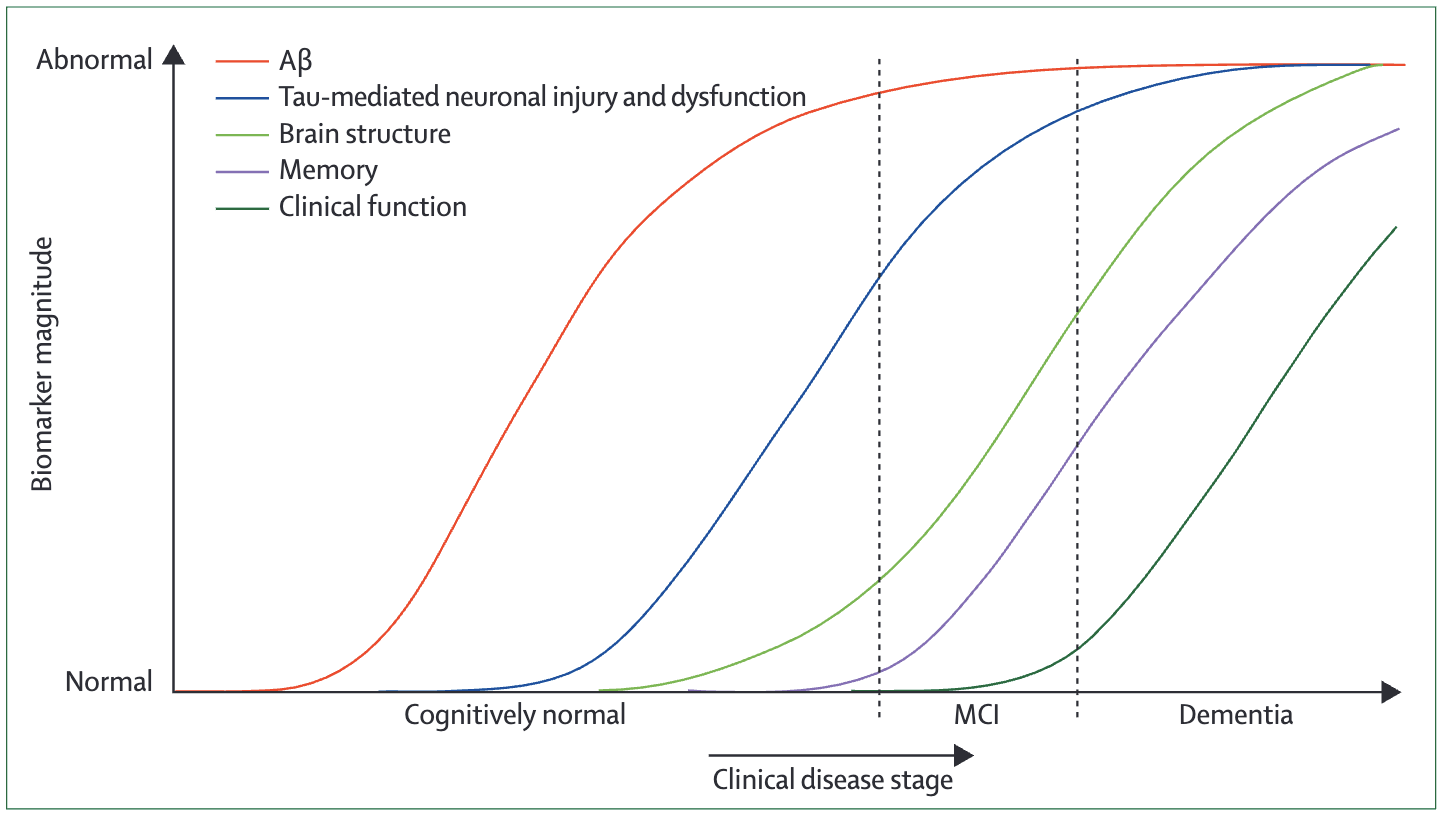
\includegraphics[width=\textwidth]{figures/biomarkers.png}
  \caption{Temporal progression of AD biomarkers, showing the relative timeline of pathophysiological changes~\cite{jack2013tracking}.}
  \label{fig:biomarker_progression}
\end{figure}

\subsubsection{Hippocampal Atrophy as Primary Biomarker}

Hippocampal atrophy represents one of the earliest and most established structural biomarkers in Alzheimer's disease progression~\cite{jack1992mr}. Volume reductions follow a predictable pattern, beginning years before clinical symptoms emerge, with annual atrophy rates of 3-6\% in AD compared to 1-2\% in normal aging~\cite{vemuri2010role}. Volumetric measurements correlate strongly with cognitive decline and Braak staging of neurofibrillary pathology. Standardized quantification methods include manual tracing, automated segmentation, and shape analysis, achieving diagnostic sensitivities of 80-90\% and specificities of 80-95\% in distinguishing AD from healthy controls~\cite{cuingnet2011automatic}.

\subsubsection{Additional Neuroimaging Markers}

Beyond volumetric measurements, shape analysis methods capture morphological changes in brain structures~\cite{ferrarini2006shape}, detecting subtle deformations missed by volume alone. Other promising markers include cortical thickness measurements~\cite{gutierrez2009patterns}, white matter integrity via diffusion tensor imaging, functional connectivity patterns, and metabolic alterations detectable through PET imaging~\cite{vemuri2010role}. These diverse markers provide complementary information that may enhance transfer learning models' diagnostic accuracy.

\subsubsection{Current Clinical Diagnostic Practices and Limitations}

Current AD diagnosis follows NINCDS-ADRDA criteria, integrating clinical assessment, cognitive testing, and biomarker analysis~\cite{dubois2007research}. Visual assessment of neuroimaging suffers from significant inter-reader variability, with diagnostic accuracy dependent on radiologist expertise~\cite{cuingnet2011automatic}. A substantial temporal gap exists between initial pathological changes and clinical manifestation, complicating early intervention~\cite{jack2018nia}. Additionally, clinical diagnostic accuracy ranges from 65-96\%, with lower precision in early disease stages when intervention would be most beneficial~\cite{kloppel2008accuracy}.

\subsubsection{Role of Structural MRI and T1-weighted Imaging in Diagnosis}

Structural MRI provides objective evidence of neurodegeneration that complements clinical assessment, with hippocampal atrophy serving as a primary biomarker~\cite{dubois2007research}. MRI's advantages include non-invasiveness compared to CSF sampling, absence of radiation exposure unlike PET, wider availability, and lower cost~\cite{vemuri2010role}. However, visual assessment suffers from inter-reader variability and limited sensitivity to subtle changes, with accuracy heavily dependent on radiologist expertise~\cite{kloppel2008accuracy}. These limitations underscore the need for quantitative, automated analysis approaches.
T1-weighted imaging offers optimal gray/white matter contrast that enhances visualization of atrophy patterns characteristic of AD~\cite{herrera2013classification}. The standardized MPRAGE protocol ensures consistent acquisition parameters across centers, facilitating algorithm development. T1-weighted sequences are widely available in clinical settings, requiring shorter acquisition times than specialized alternatives while providing excellent anatomical detail for detecting subtle volumetric changes in regions affected early in disease progression.

\subsection{Deep Learning for Medical Image Analysis}

\subsubsection{Evolution from Traditional ML to Deep Learning}

Machine learning approaches for neuroimaging have evolved dramatically over the past decade~\cite{bari2021comparative}. Early methods relied on hand-crafted features and shallow classifiers such as Support Vector Machines (SVMs), requiring extensive domain knowledge for feature engineering~\cite{cuingnet2011automatic}. These approaches typically processed predefined regions of interest, achieving moderate success but lacking generalizability. The shift to deep learning eliminated manual feature extraction, allowing end-to-end learning directly from volumetric data~\cite{litjens2017survey}. This transition has yielded substantial performance improvements, with convolutional neural networks demonstrating superior classification accuracy while requiring less preprocessing and domain expertise. The evolution reflects a fundamental shift from explicit feature definition to automatic hierarchical feature learning.

\subsubsection{2D vs. 3D Approaches for Volumetric Data}

The analysis of volumetric MRI data presents a fundamental trade-off between 2D and 3D approaches. Two-dimensional methods process brain scans as independent slices, offering computational efficiency and leveraging established architectures pretrained on natural images~\cite{liang2021alzheimer, sarraf2016classification}. However, these approaches inevitably lose spatial context between slices, potentially missing subtle 3D patterns crucial for AD detection~\cite{gunawardena2017applying}. Conversely, 3D CNNs preserve volumetric relationships and capture the entire spatial context of atrophy patterns~\cite{payan2015predicting}, but require substantially more parameters and memory~\cite{yang2021reinventing}. This computational burden necessitates downsampling in resource-constrained environments, creating a direct trade-off between spatial resolution and contextual information preservation.

Table~\ref{tab:2d_vs_3d} summarizes the key trade-offs between 2D and 3D approaches for volumetric neuroimaging analysis.

\begin{table}[htbp]
\centering
\begin{tabular}{|p{3cm}|p{6cm}|p{6cm}|}
\hline
\textbf{Aspect} & \textbf{2D Approaches} & \textbf{3D Approaches} \\
\hline
Memory Efficiency & High; processes individual slices & Low; requires full volume in memory \\
\hline
Spatial Context & Limited to in-slice patterns & Preserves volumetric relationships \\
\hline
Pre-trained Models & Readily available from natural image domains & Limited availability, primarily from video domains \\
\hline
Computational Cost & Lower training and inference times & Higher computational demands \\
\hline
Resolution & Can process higher in-plane resolution & Often requires downsampling \\
\hline
Performance & Moderate, particularly with ensemble approaches & Superior when sufficient data and computational resources are available \\
\hline
\end{tabular}
\caption{Comparison of 2D and 3D approaches for volumetric neuroimaging analysis}
\label{tab:2d_vs_3d}
\end{table}

\subsubsection{Transfer Learning in Medical Imaging}

Transfer learning addresses data scarcity in medical imaging by leveraging knowledge from models pretrained on large datasets~\cite{hon2017towards}. This approach is particularly valuable for neuroimaging applications where annotated data is limited~\cite{ebrahimi2019transfer}. When applying transfer learning to medical domains, researchers must navigate significant domain shifts between natural images and medical scans~\cite{mehmood2021transfer}.

Transfer learning strategies for medical imaging include:
\begin{enumerate}
\item \textbf{Natural image transfer:} Models pretrained on ImageNet are adapted to 2D medical slices~\cite{maqsood2019transfer}.
\item \textbf{Cross-modality transfer:} Knowledge from one imaging modality is transferred to another~\cite{yang2020mri, kieselmann2021cross}.
\item \textbf{Video-to-volumetric transfer:} Models pretrained on video datasets are adapted to 3D medical volumes~\cite{wu20223d}.
\item \textbf{Self-supervised pretraining:} Models are pretrained on unlabeled medical data using proxy tasks~\cite{tang2022self}.
\end{enumerate}

For Alzheimer's detection, researchers have explored ImageNet pretrained models using 2D slice-based methods~\cite{hon2017towards,maqsood2019transfer}, and more recently, 3D volumetric techniques with transfer from video classification models~\cite{ebrahimi2020introducing}, which shows promise due to architectural parallels between spatiotemporal video data and volumetric MRI.

To adapt pretrained models, early layers are frozen to retain low-level features while fine-tuning deeper layers for domain-specific patterns~\cite{acharya2021alzheimer}. The effectiveness of different freezing strategies depends on the similarity between source and target domains.

\subsubsection{Challenges in Deep Learning for Medical Imaging}

Deep learning approaches for medical imaging face several challenges compared to natural image analysis. Data scarcity is a primary limitation, with medical datasets typically orders of magnitude smaller than natural image collections~\cite{litjens2017survey}. This is exacerbated in neuroimaging where patient cohorts are smaller and annotation requires expertise. Also, most neuroimaging datasets are collected at specialized centers, leading to potential dataset bias.

Class imbalance presents another obstacle, particularly in Alzheimer's datasets where diagnostic categories are often unevenly distributed~\cite{davatzikos2019machine}. Clinical deployment demands model interpretability beyond accuracy metrics, as clinicians require transparency in decision-making processes. Explicable AI methods attempt to address this by identifying brain regions contributing to model decisions.

Validation protocols in neuroimaging require particular attention to prevent data leakage through subject-level rather than scan-level partitioning, an issue frequently overlooked in published studies~\cite{litjens2017survey}.

\subsection{3D Deep Learning Architectures}

\subsubsection{3D CNN Architectures (ResNet and Variants)}

3D CNNs extend convolutional operations to volumetric data, preserving spatial relationships across all dimensions critical for detecting subtle neuroanatomical changes in AD~\cite{ebrahimi2020introducing}. Early on, succesful 3D convolutional autoencoders for Alzheimer's classification established the value of learning hierarchical spatial features directly from volumetric data~\cite{payan2015predicting}. Residual networks address the vanishing gradient problem through identity shortcuts, enabling deeper architectures beneficial for capturing hierarchical patterns in volumetric MRI~\cite{wu20223d}. 3D ResNet-18 represents an optimal balance between depth and computational efficiency, containing 33.2M parameters compared to 46.4M in ResNet-34~\cite{ebrahimi2020introducing}. Architectural variants, compared in figure \ref{fig:cnn_architectures}, include MC3 (mixed 2D/3D convolutions) and R(2+1)D (factorizing 3D convolutions into spatial and temporal components, figure \ref{fig:2plus1D}) that maintain performance while reducing computational demands~\cite{wu20223d}. R3D preserves full spatial context across all dimensions, while MC3 and R(2+1)D offer computational efficiency with different approaches to dimensional processing~\cite{tran2018closer}.

\begin{figure}[htbp]
  \centering
  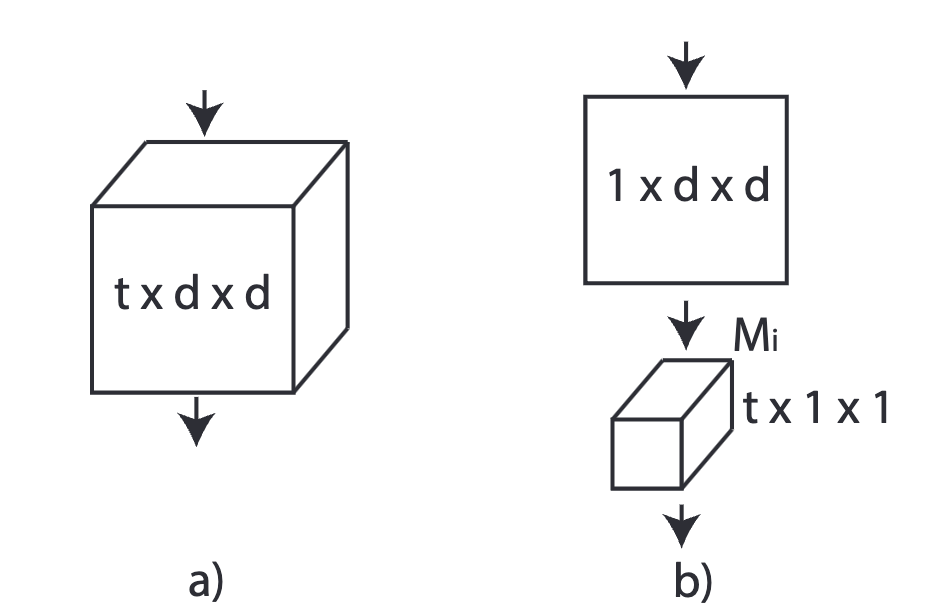
\includegraphics[width=0.5\textwidth]{figures/2plus1d.png}
  \caption{Schematic of R(2+1)D factorized convolutions. (a) being usual 3d convolutions, (b) the R(2+1)D convolutions~\cite{tran2018closer}.}
  \label{fig:2plus1D}
\end{figure}

\begin{figure}[htbp]
  \centering
  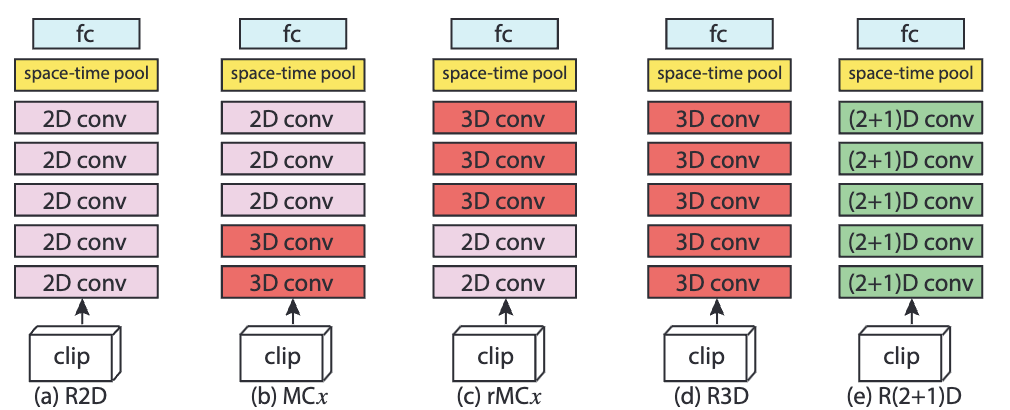
\includegraphics[width=\textwidth]{figures/res_net_archs.png}
  \caption{Schematic comparison of ResNet architectures. We will focus on (a) R3D (fully 3D convolutions), (b) MC3 (mixed 2D/3D convolutions), and (c) R(2+1)D (factorized convolutions)~\cite{tran2018closer}.}
  \label{fig:cnn_architectures}
\end{figure}

\subsubsection{Vision Transformers for Volumetric Data}

Vision Transformers (ViTs) have been adapted to volumetric medical imaging by extending self-attention mechanisms to capture 3D spatial relationships~\cite{lyu2022classification}. Yan et al. demonstrated that hybrid architectures combining CNN and transformer components (Hybrid-RViT) leverage both local feature extraction and global context modeling, outperforming pure CNN or transformer approaches for Alzheimer's detection~\cite{yan2025hybrid}. Despite their capacity to model long-range dependencies, volumetric transformers face computational challenges due to quadratic complexity with input size. Recent efficient transformer variants address these limitations through sparse attention patterns and hierarchical designs~\cite{lu2025efficient}.

Table~\ref{tab:architecture_comparison} compares key architectural approaches for volumetric neuroimaging analysis.

\begin{table}[htbp]
\centering
\begin{tabular}{|p{3cm}|p{5cm}|p{5cm}|}
\hline
\textbf{Architecture} & \textbf{Advantages} & \textbf{Limitations} \\
\hline
3D ResNet & Well-established, efficient parameter usage, strong local feature extraction & Limited receptive field, may miss long-range relationships \\
\hline
MC3 & Balance of efficiency and performance, effective knowledge transfer from video domain & Primarily captures local features, limited global context \\
\hline
R(2+1)D & Increased non-linearities through factorized convolutions, parameter efficiency & Additional computational overhead from factorization \\
\hline
Vision Transformer & Excellent global context modeling, captures long-range dependencies & High computational cost, requires large datasets \\
\hline
Hybrid CNN-ViT & Combines local feature extraction with global context modeling & Complex architecture, more hyperparameters to tune \\
\hline
\end{tabular}
\caption{Comparison of architectural approaches for volumetric neuroimaging analysis}
\label{tab:architecture_comparison}
\end{table}

\subsubsection{Video Classification Models and Medical Adaptation}

The conceptual similarity between video sequences and volumetric medical data enables innovative transfer learning approaches. In videos, the temporal dimension captures motion patterns, while in 3D MRI, the depth dimension encodes spatial relationships~\cite{tran2018closer}. Models like MC3, R(2+1)D, and r3d\_18 pre-trained on large video datasets like Kinetics-400 can be fine-tuned for MRI classification by treating the axial dimension as analogous to time~\cite{ebrahimi2020introducing, tran2018closer}.

The adaptation process requires careful consideration of domain differences. Motion patterns in videos have no direct relation to static MRI volumes, necessitating fine-tuning strategies that adapt pretrained feature extractors to the neuroimaging domain.

\subsubsection{Performance Comparisons from Existing Literature}

Benchmark studies show considerable variation in reported performance metrics. Cuingnet et al.'s seminal comparison demonstrated sensitivity ranging from 67-81\% and specificity from 68-95\% for AD versus controls using the ADNI dataset~\cite{cuingnet2011automatic}. More recent deep learning approaches report substantially higher accuracy (85-98\%), with 3D CNN architectures generally outperforming 2D approaches when properly validated~\cite{basaia2019automated, garg2023review}.

However, critical methodological analyses have revealed that many studies suffer from data leakage through scan-level rather than subject-level partitioning, potentially inflating performance by 10-15\%~\cite{davatzikos2019machine}. When accounting for proper subject isolation, performance metrics typically show more modest improvements over traditional methods.

\subsection{MRI Preprocessing for Deep Learning}

\subsubsection{Skull Stripping and Registration Approaches}

Skull stripping, the isolation of brain tissue from surrounding structures, represents a critical preprocessing step~\cite{fatima2020state}. Learning-based approaches like SynthStrip demonstrate superior robustness across imaging protocols and pathological conditions~\cite{hoopes2022synthstrip}. SynthStrip particularly excels with neurodegenerative cases, where traditional methods like intensity-based thresholding often fail due to enlarged ventricles and cortical atrophy, see figure \ref{fig:skull_stripping}.

\begin{figure}[htbp]
  \centering
  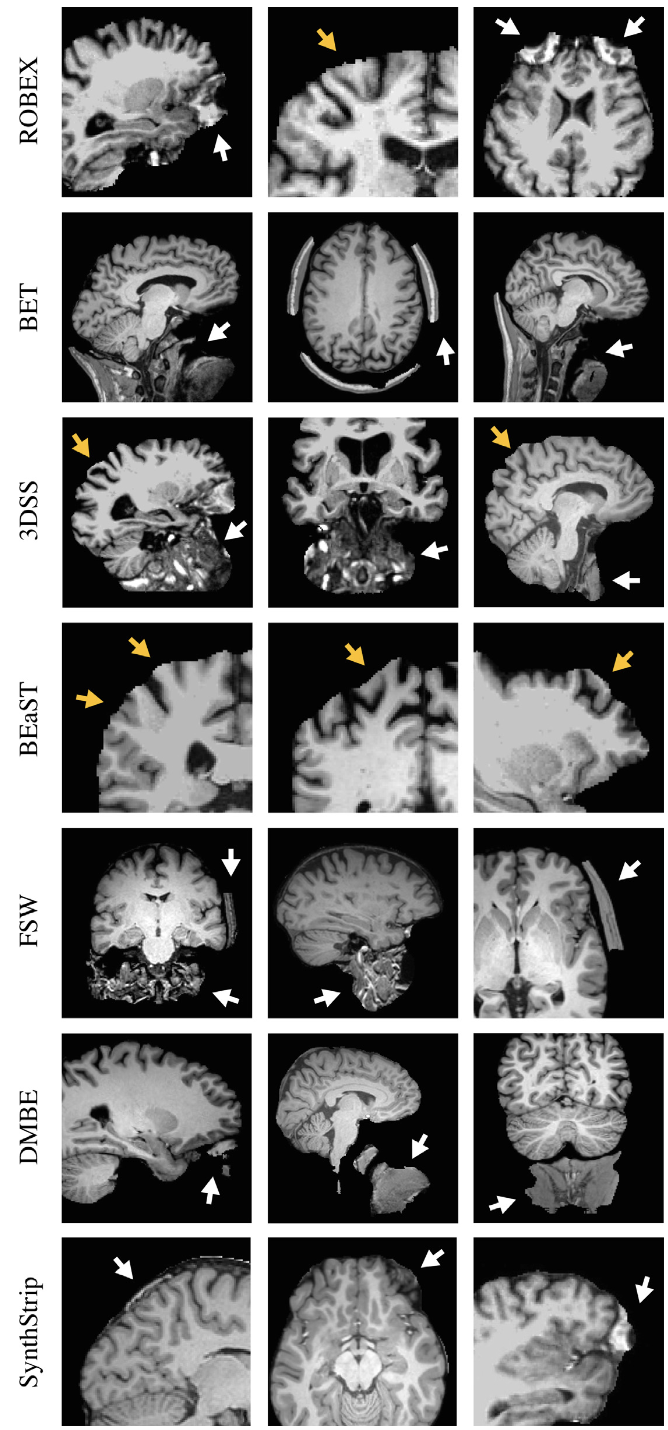
\includegraphics[width=0.33\textwidth]{figures/ss_fails.png}
  \caption{Example of common failures of skull stripping methods. We can see how the minor mistakes synthstrip commits do not crop the brain structure like more primitive methods do~\cite{hoopes2022synthstrip}}
  \label{fig:skull_stripping}
\end{figure}

Registration to standardized templates (e.g., MNI152) normalizes anatomical variability, facilitating voxel-wise comparisons across subjects~\cite{garg2023review}. However, registration presents a trade-off between standardization and preservation of pathology-specific features. While traditional machine learning approaches typically benefit from rigorous registration, deep learning methods can achieve superior performance with minimal registration that preserves native anatomical features by learning invariant representations, potentially extracting diagnostic patterns despite anatomical variability.

While normalization improves model interpretability by establishing spatial correspondence~\cite{viswan2025enhancing}, excessive regularization risks attenuating the volumetric changes characteristic of AD. Intensity normalization addresses scanner-specific variations, with Z-score normalization particularly effective for deep learning applications by constraining gradient magnitudes during training~\cite{viswan2025enhancing}.

\subsubsection{Impact of Preprocessing on Model Performance}

Preprocessing significantly impacts deep learning performance for AD detection. Viswan et al. demonstrated that proper preprocessing pipelines can improve classification accuracy by 5-15\% compared to minimal preprocessing~\cite{viswan2025enhancing}. Skull stripping shows the most substantial impact, with improperly stripped volumes reducing accuracy by up to 8\%. Registration demonstrates a more nuanced effect—while standardizing anatomical positioning enhances performance for shallow classifiers, deep networks can sometimes perform better with unregistered data preserving native atrophy patterns. Intensity normalization consistently improves performance by 3-7\% across architectures by mitigating scanner variability.

Table~\ref{tab:preprocessing_impact} summarizes the impact of different preprocessing steps on model performance.

\begin{table}[htbp]
\centering
\begin{tabular}{|p{3cm}|p{5cm}|p{5cm}|p{2cm}|}
\hline
\textbf{Preprocessing Step} & \textbf{Implementation Approach} & \textbf{Effect on Performance} & \textbf{Relative Impact} \\
\hline
Skull Stripping & Learning-based (SynthStrip) & Eliminates confounding signals, improves feature extraction precision & High (+5-8\%) \\
\hline
Registration & Affine only (preserving some atrophy patterns) & Standardizes orientation while preserving disease-specific features & Moderate (+2-5\%) \\
\hline
Intensity Normalization & Z-score normalization & Mitigates scanner variability, constrains gradient magnitudes & Moderate (+3-7\%) \\
\hline
Bias Field Correction & N4 algorithm & Reduces intensity non-uniformity artifacts & Low-Moderate (+1-3\%) \\
\hline
\end{tabular}
\caption{Impact of preprocessing steps on model performance for AD classification}
\label{tab:preprocessing_impact}
\end{table}

\subsection{Data Partitioning and Group Leakage Prevention}
\label{subsec:data_partitioning}

Data leakage represents a critical methodological concern in neuroimaging studies, occurring when information from test samples inadvertently influences model training. This issue is particularly problematic in longitudinal neuroimaging datasets with multiple scans from the same subject across different timepoints~\cite{davatzikos2019machine}.

Subject-level partitioning—ensuring all scans from an individual remain exclusively in either training, validation, or test sets—is essential for preventing "group leakage." In contrast, scan-level partitioning (where different scans from the same subject may appear in both training and test sets) can dramatically overestimate model performance by 10-15\% in classification accuracy~\cite{davatzikos2019machine}.

Many published neuroimaging studies fail to clearly report their data partitioning methodology, making it difficult to assess the validity of reported performance metrics. This has led to a growing emphasis on methodological transparency and rigorous validation protocols in recent literature~\cite{davatzikos2019machine}.

\subsection{Current State of the Art and Research Gaps}

\subsubsection{Recent Advances in Automated AD Detection}

Recent years have seen significant progress in automated Alzheimer's disease detection using deep learning. Convolutional neural networks have emerged as the dominant methodology, with 3D architectures demonstrating superior performance. Early approaches achieved strong accuracy using 2D CNN ensembles~\cite{farooq2017deep}, then transfer learning to 3D ResNet-18 was introduced, leveraging pre-trained weights to achieve 96.88\% accuracy despite limited training data~\cite{ebrahimi2020introducing}.Vision Transformers (ViTs) represent the newest architectural innovation, with hybrid CNN-transformer models demonstrating state-of-the-art performance. Current performance benchmarks for binary AD classification range from 85-98\% accuracy, with 3D approaches consistently outperforming 2D counterparts~\cite{saikia2024alzheimer,mubonanyikuzo2025detection}. However, it is unclear whether these account for proper subject-level validation.

Despite these advances, several challenges remain. Data scarcity limits model training~\cite{pradhan2024analysis}, while heterogeneous MRI acquisition protocols introduce variability that complicates model generalization. Adapting video classification architectures to 3D MRI data requires substantial modifications that may compromise the benefits of pre-trained weights. The "black box" nature of deep learning models raises concerns about clinical interpretability and trustworthiness~\cite{basaia2019automated}. Lastly, domain shift between source and target tasks remains problematic, potentially limiting the effectiveness of knowledge transfer from non-medical to medical imaging applications.

\subsubsection{Research Gap Addressed by This Work}

Despite advances in deep learning for Alzheimer's detection, several key methodological and technical gaps remain that this work aims to address:

\begin{enumerate}
\item \textbf{Volumetric transfer learning:} The adaptation of pretrained 3D models for volumetric medical imaging remains underexplored. This work systematically investigates the effectiveness of video-pretrained models for AD classification.

\item \textbf{Methodological rigor:} Many published studies suffer from methodological flaws including scan-level partitioning. This research implements rigorous subject-level validation methodology.

\item \textbf{Preprocessing optimization:} The impact of different preprocessing choices on transfer learning performance is incompletely understood. This work develops an optimized pipeline specifically designed to preserve diagnostically relevant features.

\item \textbf{Architectural comparison:} Limited research exists comparing architectures specifically optimized for video classification on neuroimaging tasks. This study evaluates these variants to determine the optimal approach for volumetric MRI analysis.
\end{enumerate}

These research gaps directly inform the methodology in the next section, which implements a rigorous experimental framework to evaluate video-pretrained model transfer for Alzheimer's disease detection.

\section{Methodology}
% 2,500 words

\subsection{Data Acquisition and Characteristics}

The Alzheimer's Disease Neuroimaging Initiative (ADNI) database served as the primary data source, providing standardized MRI acquisitions with corresponding clinical diagnoses. ADNI was selected over alternatives (including OASIS) for its comprehensive coverage, acquisition protocols, and expert-validated diagnoses~\cite{jack2008alzheimer, lamontagne2019oasis}.

\subsubsection{Dataset Composition}

All selected scans were T1-weighted MPRAGE sequences (1.5T or 3T, 1mm³ isotropic resolution), chosen for optimal gray/white matter contrast, standardized acquisition parameters, and sensitivity to atrophy biomarkers. Additionally, the widespread clinical availability and established role of MPRAGE in AD assessment made it an ideal choice for this study. The final dataset contained 1,300 scans from 408 unique subjects, balanced between diagnostic categories:

\begin{table}[htbp]
\centering
\begin{tabular}{|l|c|c|}
\hline
\textbf{Partition} & \textbf{AD} & \textbf{CN} \\
\hline
Training & 512 scans (133 subjects) & 511 scans (115 subjects) \\
Validation & 69 scans (35 subjects) & 70 scans (45 subjects) \\
Test & 69 scans (35 subjects) & 69 scans (45 subjects) \\
\hline
\end{tabular}
\caption{Distribution of scans and subjects across dataset partitions}
\end{table}

\subsubsection{Diagnostic Criteria}

Subjects were classified as Alzheimer's Disease (AD) or Cognitively Normal (CN) based on NINCDS-ADRDA criteria. Initially, the dataset contained approximately 33\% AD and 67\% CN cases. To address class imbalance and potential overfitting issues identified during preliminary experiments, additional AD scans were incorporated and CN subjects carefully sampled to achieve a balanced 50/50 diagnostic distribution.

The binary classification focus (excluding Mild Cognitive Impairment) reflects the clearer structural changes observable in established AD, particularly hippocampal atrophy, which serves as a primary biomarker for disease progression. Subject-level isolation between dataset partitions was strictly enforced to prevent data leakage, ensuring realistic performance assessment for unseen individuals.

\subsection{Preprocessing Pipeline}

\subsubsection{Initial Processing and Skull Stripping}

Raw DICOM images were converted to NIfTI format using \texttt{dicom2nifti} with reorientation and compression enabled. This created unified volumetric files suitable for 3D analysis. Skull stripping was performed using SynthStrip, a deep learning-based method that represents the current state-of-the-art for brain extraction~\cite{hoopes2022synthstrip}. It was selected for its superior performance with atrophied brains. Unlike traditional threshold-based methods (e.g., BET), SynthStrip preserved critical cortical boundaries even with atrophied brains and better handled the variability in the ADNI dataset. Despite requiring ~2.5 minutes per scan, the improved quality justified this approach by preventing potential misinterpretation of artifacts as disease-related changes.

\subsubsection{Volume Standardization}

All volumes were resampled to isotropic 1×1×1mm voxels using ANTs with third-order spline interpolation. This standardization ensured consistent spatial representation, eliminated scanner-specific resolution variability, and enabled uniform convolutional filter operations across all dimensions.

\subsubsection{Adaptive Cropping Strategy}

A key methodological innovation was the implementation of an adaptive cropping procedure followed by reshaping to 128×128×128 dimensions. The approach:

\begin{enumerate}
    \item Identified brain-containing regions using intensity thresholding
    \item Applied cropping with minimal padding (3 voxels)
    \item Used cubic interpolation to reach the target dimensions
\end{enumerate}
% TODO add appendix to crop brain from mri function

This method preserved approximately 35\% more effective resolution for critical structures like the hippocampus compared to naive downsampling. The 128³ dimension balanced preserving anatomical detail with memory constraints for model training. The original uncropped 96³ images compared to the cropped 128³ images are shown in figure \ref{fig:cropping}.
\begin{figure}[htbp]
  \centering
  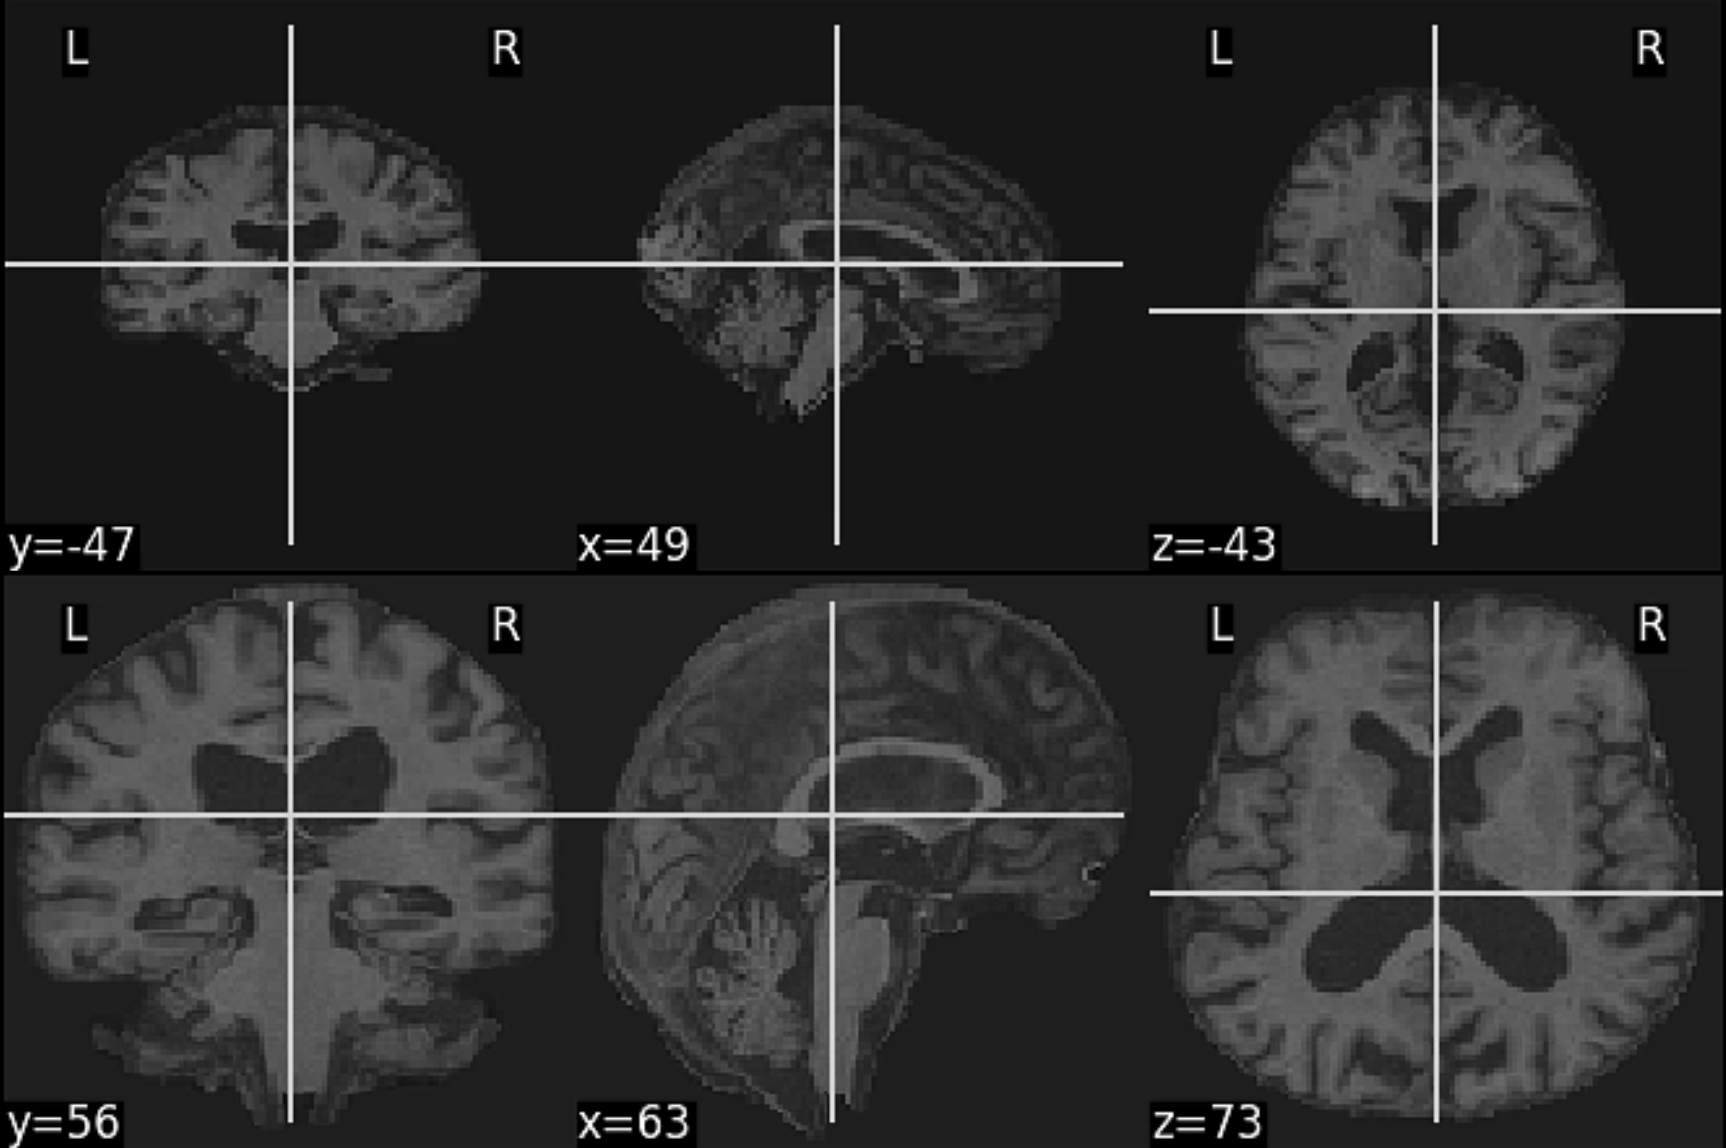
\includegraphics[width=0.8\textwidth]{figures/cropping.png}
  \caption{Comparison of original 96³ (top) and cropped 128³ (bottom) images. The cropping process preserves critical anatomical features while reducing irrelevant background.}
  \label{fig:cropping}
\end{figure}

\subsubsection{Intensity Normalization and Orientation}

N4 bias field correction was applied to mitigate intensity inhomogeneities from magnetic field variations. This prevents intensity variations that might be misinterpreted as structural changes. All volumes were reoriented to Right-Anterior-Superior (RAS) orientation to ensure consistent directionality, allowing the model to focus solely on relevant structural differences rather than arbitrary orientation variations.
% TODO reference code from appendix

\subsubsection{Omission of Spatial Normalization}

Despite its common use in neuroimaging pipelines, registration to standard space (e.g., MNI152) was deliberately omitted for several reasons:
\begin{enumerate}
    \item Preservation of native atrophy patterns that could be distorted during normalization
    \item Reliance on CNN translation invariance to identify structures without explicit alignment
    \item Avoidance of interpolation artifacts that might smooth critical structural boundaries
    \item Computational efficiency gains without compromising classification performance
\end{enumerate}

Validation experiments confirmed that models trained on native-space data performed comparably to or better than those using normalized data, supporting this methodological decision and aligning with recent literature suggesting deep learning models for brain MRI benefit from native-space learning.

The entire pipeline produced 1,300 preprocessed volumes with consistent dimensions, orientation, and intensity characteristics while preserving the structural variations essential for AD classification.

\subsection{Data Splitting Strategy}

A methodologically rigorous data splitting approach was implemented to prevent data leakage while maintaining diagnostic balance across partitions. Unlike conventional image classification tasks, neuroimaging datasets require subject-level rather than scan-level splitting since multiple scans often exist for the same individual.

\subsubsection{Subject-Level Isolation}

A strict subject-level isolation approach ensured no individual appeared in multiple dataset partitions—a critical decision after initial experiments revealed artificially inflated performance metrics (~90\% accuracy) when subjects were allowed to cross partition boundaries. Complete subject isolation produced a more realistic performance assessment (~77\% accuracy), better reflecting the model's generalization capability to unseen individuals.

\subsubsection{Partition Distribution}

The dataset was divided following an 80/10/10 (train/validation/test) ratio using a round-robin algorithm that:
\begin{enumerate}
    \item Grouped subjects by diagnostic condition
    \item Sorted subjects in ascending order by scan count
    \item Allocated subjects to partitions round robin to insure subject diversity across partitions
    \item Final scan counts were balanced to maintain equal scan counts per diagnostic category
\end{enumerate}

This approach yielded a balanced distribution with 1,023 training scans (512 AD/511 CN), 139 validation scans (69 AD/70 CN), and 138 test scans (69 AD/69 CN). The strict isolation maintained 203 unique subjects in training, 80 in validation, and 80 in test sets, with diagnostic balance preserved in each partition.

\paragraph{Data Leakage Prevention}

To prevent subtle forms of data leakage, subject identifiers were rigorously tracked and preprocessing parameters (such as intensity normalization statistics) were computed independently within each partition. This methodologically sound approach ensured that performance metrics would accurately reflect the model's ability to generalize to entirely new individuals, rather than merely recognizing previously seen subjects in different scans.

\subsection{Data Augmentation}

Data augmentation was strategically implemented to improve model generalization while preserving diagnostically relevant features. Through systematic experimentation, a minimal yet effective set of transformations was identified:

\begin{verbatim}
tio.Compose([
    tio.RandomNoise(mean=0.0, std=0.1, p=0.3),
    tio.RandomGamma(log_gamma=(-0.2, 0.2), p=0.3),
    tio.ZNormalization(),
])
\end{verbatim}

This approach was applied exclusively to the training set, while validation and test sets received only Z-normalization to maintain evaluation consistency. In practice I saw a 5\% improvement in test accuracy, and consistent improvement in validation accuracy as seen in figure \ref{fig:normalisation_accuracy}.

Each technique addressed specific neuroimaging considerations: Random noise (30\% probability, $\sigma$=0.1) simulated scanner variability and promoted robustness to image quality differences; Gamma adjustment (±0.2 range, 30\% probability) mimicked contrast variations between scanners; Z-normalization standardized intensity values across all scans for consistent feature extraction.

Notably, several common augmentation techniques were deliberately excluded after experimental evaluation showed either no benefit or negative impact:

\begin{itemize}
    \item \textbf{Geometric transformations} (rotations, flips) significantly increased training time (~20 vs ~5 epochs) without improving validation accuracy, likely due to inherent orientation variability already present in MRI data.
    
    \item \textbf{Random scaling} (0.9-1.1) showed no generalization improvement and potentially disrupted the carefully standardized voxel dimensions.
\end{itemize}

The final strategy evolved from extensive transformations to this focused set through iterative evaluation of validation performance and convergence speed, representing an optimal balance between enhancing robustness and preserving critical structural features essential for AD classification.
\subsection{Model Architectures}
\subsubsection{3D ResNet Architecture}

The primary model was a modified 3D ResNet-18 (r3d\_18), selected for its residual connections that mitigate vanishing gradients, fully 3D convolutional operations to preserve volumetric spatial relationships, and parameter efficiency (33M parameters) enabling training on consumer hardware. The ResNet architecture family has demonstrated robust performance across numerous computer vision tasks, including medical imaging applications, and is used frequently in the literature. The implementation used PyTorch's pre-trained r3d\_18 model, with the first layer modified to accept single-channel MRI volumes and the final layer adapted for binary classification.

The model architecture consisted of 18 layers, with the first layer being a 3D convolutional layer followed by four residual blocks, each containing two 3D convolutional layers. The final fully connected layer was adapted to output binary classification scores. The model was trained using a transfer learning approach, leveraging pre-trained weights from the Kinetics400 dataset, which provided a strong initialization for the feature extraction layers.

\subsubsection{Transfer Learning Strategy}

We implemented a selective transfer learning approach, freezing early convolutional layers (25\% of parameters) while allowing the final residual block and fully connected layer (75\%) to adapt to MRI-specific features. This balanced preserving pre-trained knowledge with domain adaptation. Initial experiments with more aggressive freezing (keeping only the final fully connected layer trainable) resulted in numerical instabilities during training, manifested as NaN losses, suggesting that significant domain adaptation was necessary given the substantial differences between video action recognition and MRI classification.

A differential learning rate strategy applied a 10× higher learning rate to the newly initialized fully connected layer compared to the fine-tuned convolutional layers, enabling aggressive adaptation in the task-specific output layer while making more conservative updates to the pre-trained feature extraction layers.
% TODO add learning rates code in appendix

\subsubsection{Architecture Comparison}

To validate architectural choices, models were systematically evaluated with decreasing levels of 3D feature extraction:

\begin{enumerate}
    \item \textbf{Mixed Convolution 3D Network}: This model (MC3-18) uses a hybrid approach combining 2D and 3D convolutions, hypothesized to potentially offer computational efficiency while maintaining performance.
      
      Experimental results with MC3-18 showed less stable training dynamics and inferior performance compared to the pure 3D approach of R3D-18, supporting the importance of fully volumetric feature extraction for structural MRI analysis. The differences in performance provided empirical justification for the primary architectural choice.

    \item \textbf{(2+1)D Convolution Network}: Following the investigation of MC3-18, a (2+1)D architecture was also evaluated. This approach decomposes 3D convolutions into separate spatial (2D) and temporal (1D) convolutions, a technique that has shown promise in video classification tasks.
      
      Results with the (2+1)D architecture revealed performance that was slightly worse than MC3-18, continuing the observed trend that classification accuracy decreased as the model architecture incorporated more 2D elements. This progression (R3D > MC3 > (2+1)D) strongly suggests that preserving the full 3D spatial context through pure 3D convolutions is critical for detecting the subtle volumetric patterns associated with Alzheimer's disease in MRI data.
      
    \item \textbf{Multiscale Vision Transformer}: Recent advances in vision transformers prompted investigation of their potential for 3D MRI classification. However, initial implementation attempts revealed significant computational barriers:
      
      \begin{enumerate}
        \item Memory requirements exceeded available hardware capabilities (32GB RAM requirement for 128×128×128 volumes)
        \item Architectural mismatch between the input dimensions required by MViT (designed for 16×224×224 video clips) and the cubical 128×128×128 MRI volumes
        \item Transformer architectures typically require substantially larger training datasets than were available
      \end{enumerate}
      
      These constraints prevented full evaluation of transformer-based approaches, highlighting an important practical limitation in applying state-of-the-art vision models to medical imaging with limited computational resources.
\end{enumerate}

\subsubsection{Parameter Counts and Computational Considerations}

The final model architecture parameters were:

\begin{itemize}
    \item \textbf{Total parameters}: 33,148,482
    \item \textbf{Trainable parameters}: 24,909,826 (75.15\%)
    \item \textbf{Frozen parameters}: 8,238,656 (24.85\%)
\end{itemize}

These figures represent a significant reduction compared to larger architectures like ResNet-50 or ViT variants, making training feasible on consumer-grade hardware while maintaining sufficient capacity for the classification task. The reduced parameter count also potentially mitigated overfitting given the relatively small dataset size.

\subsection{Training Framework and Implementation}

Training was conducted on an M1 Mac using Metal Performance Shaders, with each epoch requiring approximately one hour and full training runs taking ~20 hours. This hardware constrained batch size and architecture selection. Despite attempts at optimization through mixed precision training and CPU-GPU synchronization, computational bottlenecks in the model's forward pass remained.

Hyperparameters were selected through systematic experimentation and tracked with Weights \& Biases:

\begin{table}[htbp]
\centering
\begin{tabular}{|l|l|p{5.5cm}|}
\hline
\textbf{Parameter} & \textbf{Value} & \textbf{Rationale} \\
\hline
Learning rate & 0.001 (FC), 0.0001 (conv) & Differential rates for aggressive output adaptation with conservative updates to pre-trained layers \\
\hline
Optimizer & AdamW (weight decay=0.01) & Effective regularization for the limited dataset \\
\hline
Batch size & 2 & Memory constraints from 128³ inputs \\
\hline
LR schedule & Cosine annealing ($T_0$=5) & Prevents convergence to local minima \\
\hline
\end{tabular}
\caption{Optimized hyperparameter configuration}
\end{table}

A weighted cross-entropy loss function addressed potential class imbalance with weights dynamically calculated based on class distribution, particularly important during initial experiments when the dataset had not yet been fully balanced. This ensured balanced contribution to loss regardless of class representation.

% TODO add to appendix

Early stopping with patience=5 monitored both validation accuracy and loss, ensuring training continued as long as either metric showed enhancement, preventing overfitting while optimizing computational resources. Most models converged within 5-10 epochs, with early stopping typically triggering around epoch 7-8—quick convergence attributable to the transfer learning initialization.

A comprehensive checkpoint system saved regular epoch checkpoints and best models based on both accuracy and loss metrics. Each checkpoint stored model weights, optimizer state, scheduler state, and performance metrics for seamless training resumption. The system integrated with Weights \& Biases to log best models as artifacts.

The training loop was implemented with careful attention to numerical stability and memory management. Memory optimization techniques included setting gradients to \texttt{None} rather than zero (reducing memory fragmentation) and using tensor operations that maintained computational efficiency. For MPS acceleration, explicit cache clearing was performed at the end of each epoch to prevent memory accumulation.

\subsection{Evaluation Methodology}

\subsubsection{Performance Metrics}

A comprehensive set of metrics was implemented to evaluate model performance beyond simple accuracy:

\begin{itemize}
    \item \textbf{Accuracy and balanced accuracy}: The latter particularly important for medical applications as it equalizes the contribution of each diagnostic class.
    
    \item \textbf{Precision and recall}: Critical for clinical utility, measuring correct positive predictions and the ability to identify true AD cases, respectively.
    
    \item \textbf{Specificity}: Quantified the model's ability to correctly identify CN cases ($TN/(TN+FP)$).
    
    \item \textbf{F1-score, ROC-AUC, and average precision}: Provided threshold-independent performance assessment.
\end{itemize}

All metrics were continuously tracked and logged using a custom \texttt{MetricsManager} class, with implementation details provided in Appendix X.
% TODO add to appendix

\subsubsection{Validation Strategy}

The evaluation framework employed strict subject-level isolation to prevent data leakage:

\begin{itemize}
    \item Dedicated validation (10\%) and test (10\%) sets maintained complete separation from training data.
    
    \item Multiple model checkpoints were saved (best accuracy and best loss) to mitigate selection bias.
    
    \item Final evaluation used only the held-out test set with the best validation accuracy checkpoint.
\end{itemize}

\subsubsection{Statistical Analysis}

Statistical rigor was ensured through:

\begin{itemize}
    \item Bootstrap confidence intervals for key metrics to quantify the uncertainty in performance estimates
    
    \item Confusion matrix analysis to identify classification patterns
    
    \item Comparison to baselines: random chance (50\%), clinical radiologist performance, and published algorithmic approaches
\end{itemize}

\subsubsection{Cross-Validation and Architecture Evaluation}

Despite computational constraints (20-hour training runs on M1 Mac), model robustness was verified through:

\begin{itemize}
    \item Subject-level 3-fold cross-validation with diagnostic balance and subject-level isolation maintained across all partitions.
    
    \item Systematic architecture comparison across R3D-18, MC3-18, and R2Plus1D-18 to assess the impact of dimensional processing on performance and to validate the choice of fully 3D convolutional architectures
    
    \item Visualization techniques to provide qualitative insights into model behavior, rather than relying solely on quantitative metrics
\end{itemize}

Cross-validation reveal performance consistency across subject groupings, while architectural evaluation demonstrate whether fully 3D convolutional approaches systematically outperform partial 2D/3D hybrid methods

\section{Results}
% 2,000 words

This section presents the quantitative and qualitative results of the proposed transfer learning approach for Alzheimer's disease detection using pre-trained video classification models adapted to MRI analysis. The results demonstrate the effectiveness of 3D convolutional architectures, particularly the R3D-18 model, for identifying structural patterns associated with AD.

\subsection{Overall Performance Metrics}

\subsubsection{Classification Performance}

The optimized R3D-18 model achieved a test accuracy of 77.26\% for the binary classification of AD versus CN subjects, with balanced precision and recall metrics. Table \ref{tab:performance_metrics} summarizes the key performance metrics for the final model evaluated on the held-out test set and average over each fold.

\begin{table}[htbp]
\centering
\begin{tabular}{|l|c|}
\hline
\textbf{Metric} & \textbf{Value} \\
\hline
Accuracy & 77.26\% \\
Balanced Accuracy & 77.31\% \\
Precision & 77.1\% \\
Recall (Sensitivity) & 79.29\% \\
Specificity & 75.33\% \\
F1-Score & 77.13\% \\
AUC-ROC & 0.86 \\
\hline
\end{tabular}
\caption{Performance metrics for the R3D-18 model on the held-out test set.}
\label{tab:performance_metrics}
\end{table}

The confusion matrix in Figure \ref{fig:confusion_matrix} shows the distribution of predictions across diagnostic categories, revealing a balanced performance between AD and CN classifications with similar false positive and false negative rates.

\begin{figure}[htbp]
  \centering
  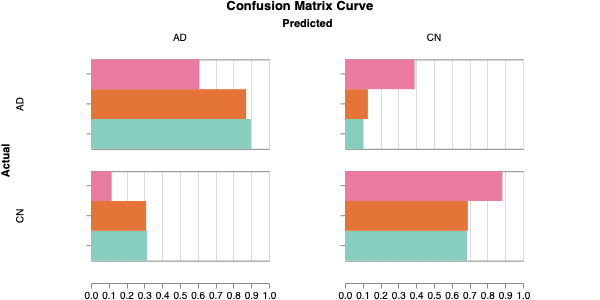
\includegraphics[width=\textwidth]{figures/CM3F.png}
  \caption{Confusion matrix for AD vs CN classification on the test set over 3 folds, showing the distribution of true positives, false positives, true negatives, and false negatives.}
  \label{fig:confusion_matrix}
\end{figure}

\subsubsection{ROC Analysis}

The Receiver Operating Characteristic (ROC) curve in Figure \ref{fig:roc_curve} demonstrates the trade-off between true positive rate and false positive rate across different classification thresholds. With an Area Under the Curve (AUC) of 0.86, it indicates good discriminative ability between AD and CN subjects.

\begin{figure}[htbp]
  \centering
  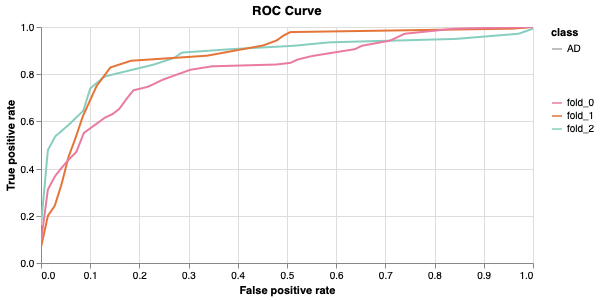
\includegraphics[width=\textwidth]{figures/ROC3F.png}
  \caption{ROC curve for the R3D-18 model on the held out test set over 3 folds. The Area Under the Curve (AUC) is 0.86.}
  \label{fig:roc_curve}
\end{figure}

\subsubsection{Cross-Validation Stability}

To assess model stability and generalization, we performed 3-fold cross-validation with strict subject-level isolation maintained across folds. The results in Table \ref{tab:cross_validation} demonstrate consistent performance across different subject groupings, with a mean accuracy of 77.26\% and standard deviation of 2.34\%.

\begin{table}[htbp]
\centering
\begin{tabular}{|c|c|c|c|c|}
\hline
\textbf{Metric} & \textbf{Fold 1} & \textbf{Fold 2} & \textbf{Fold 3} & \textbf{Mean ± SD} \\
\hline
Accuracy & 79.1\% & 78.01\% & 74.64\% & 77.26 ± 2.34\% \\
\hline
Precision & 73.81\% & 73.49\% & 84.00\% & 77.1 ± 5.98\% \\
\hline
Recall & 89.86\% & 87.14\% & 60.87\% & 79.29 ± 16.01\% \\
\hline
F1-Score & 81.05\% & 79.74\% & 70.59\% & 77.13 ± 5.70\% \\
\hline
\end{tabular}
\caption{3-fold cross-validation results demonstrating model stability across different subject groupings.}
\label{tab:cross_validation}
\end{table}

The low standard deviation (2.34\%) across folds indicates robust performance independent of specific subject allocation, supporting the generalizability of our approach to unseen individuals.

\subsubsection{Learning Curve Analysis}

The learning curves for the R3D-18 model over 3 folds exhibited relatively quick convergence, typically within 4-8 epochs, attributable to the transfer learning initialization. Figure \ref{fig:learning_curves} shows the characteristic progression of training and validation metrics across epochs.

\begin{figure}[htbp]
  \centering
  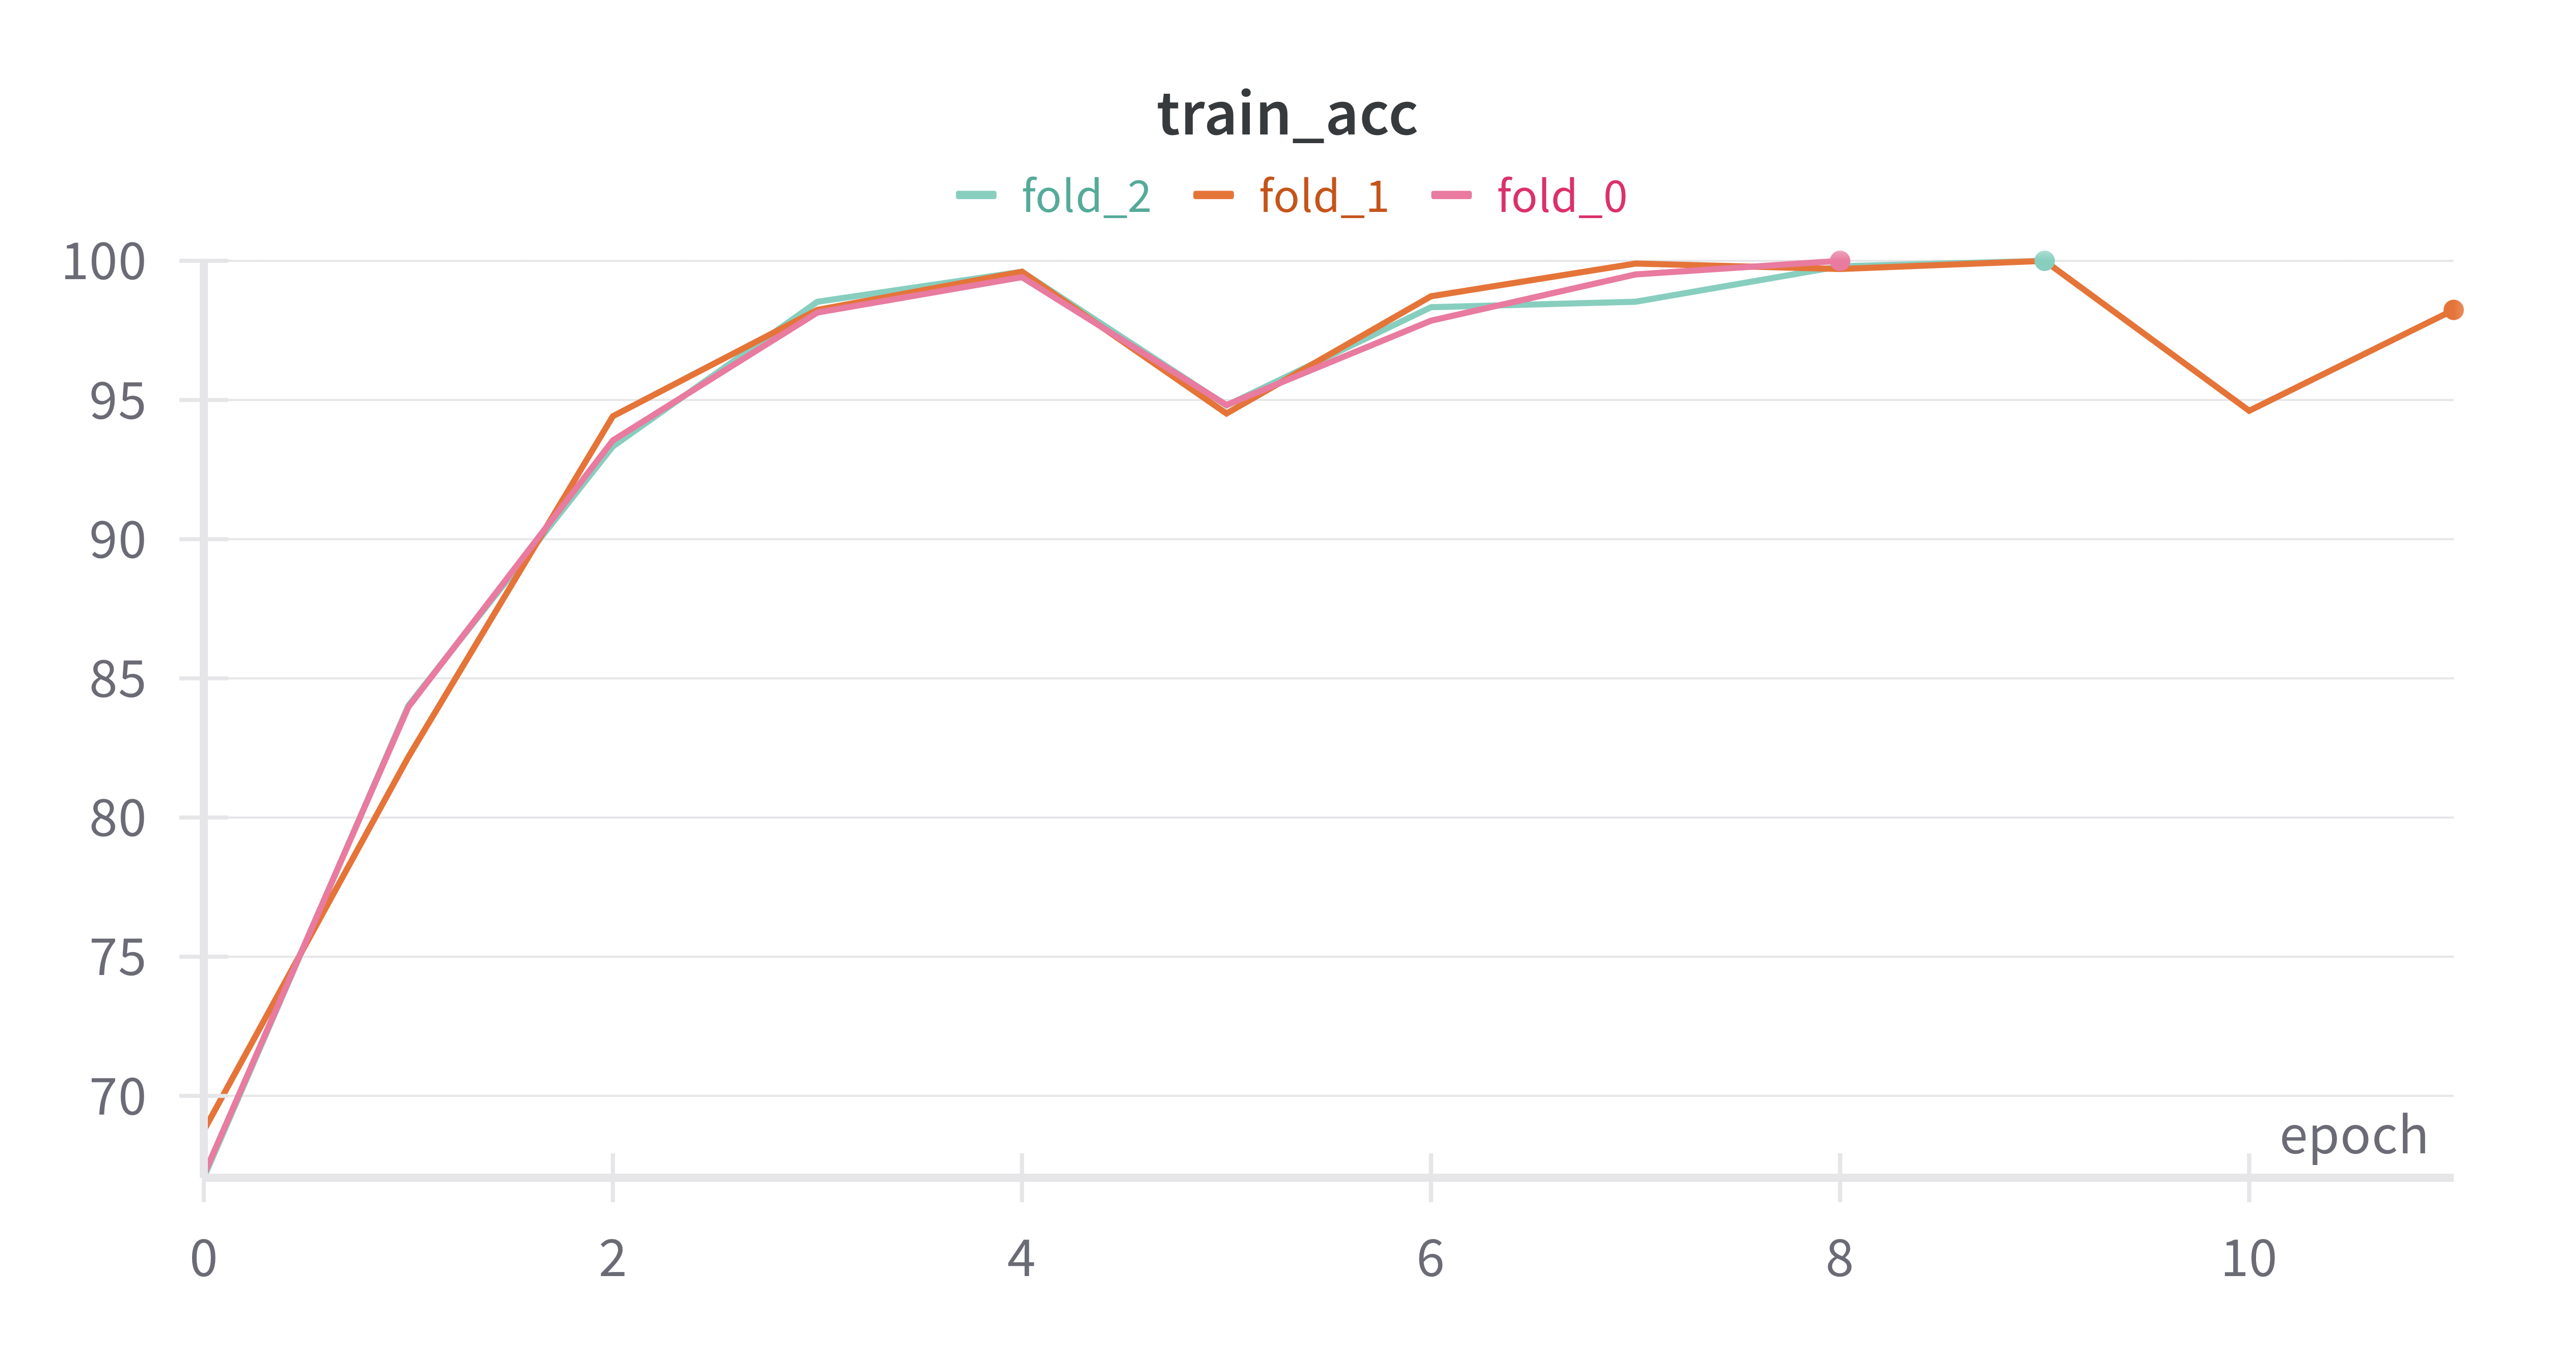
\includegraphics[width=0.6\textwidth]{figures/3f_train_acc.png}
  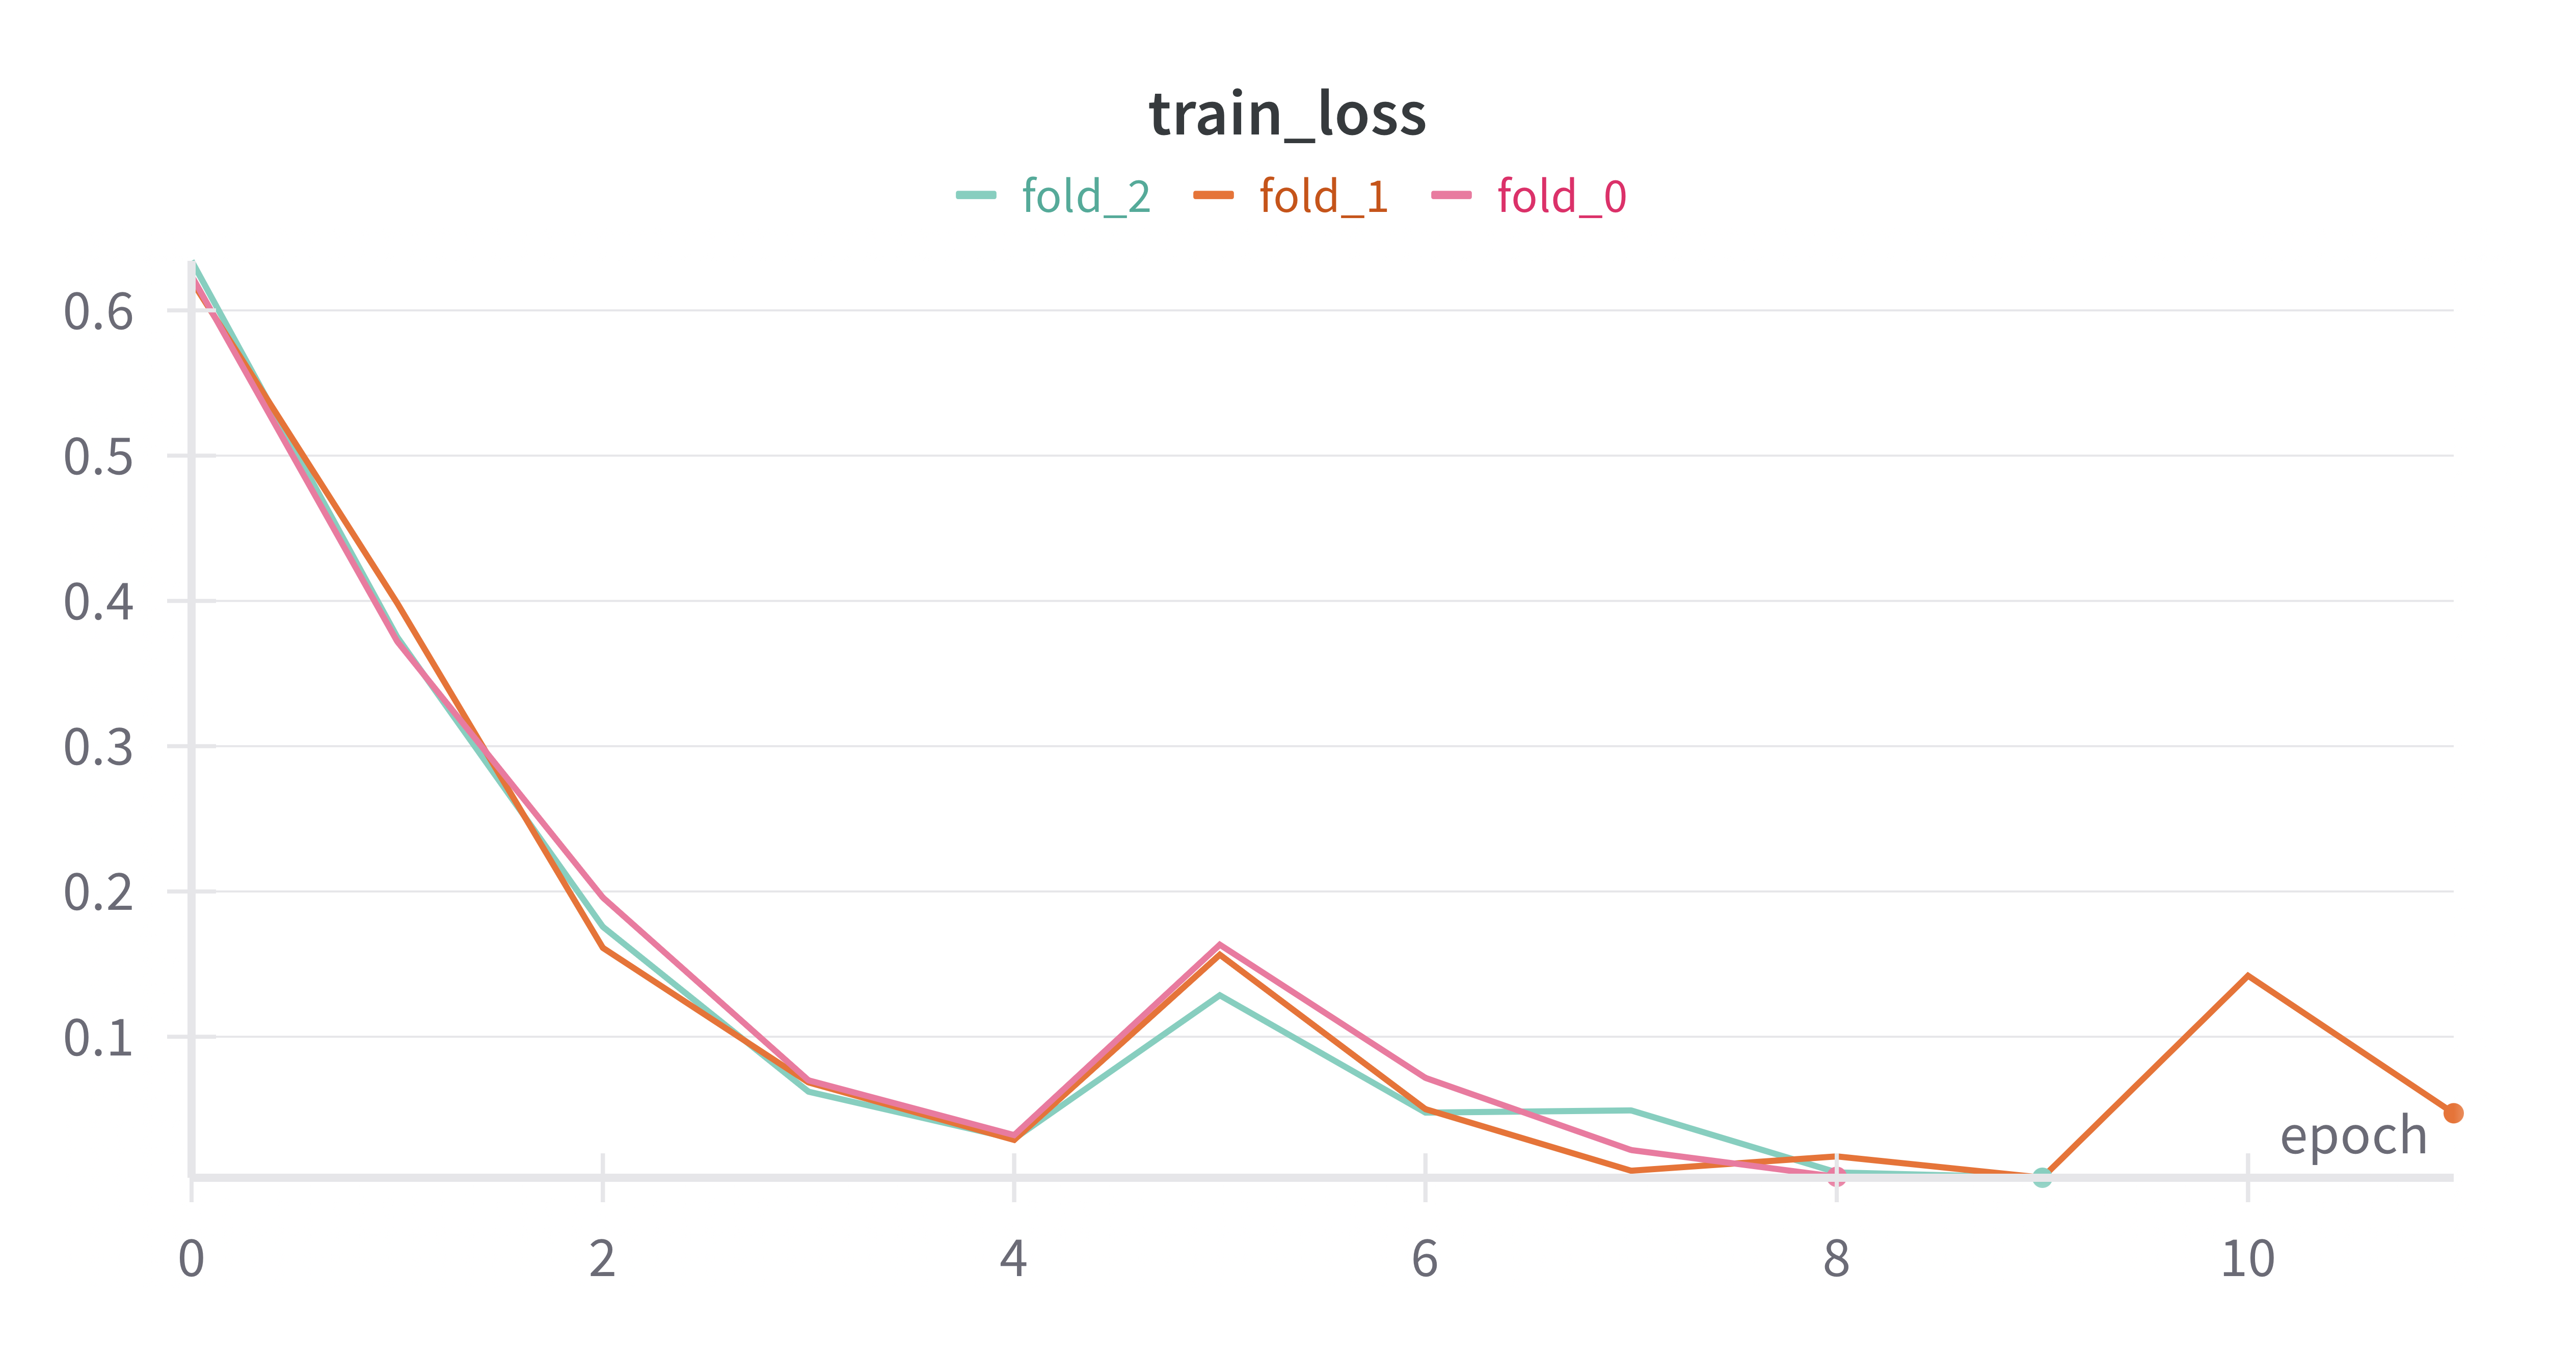
\includegraphics[width=0.6\textwidth]{figures/3f_train_loss.png}
  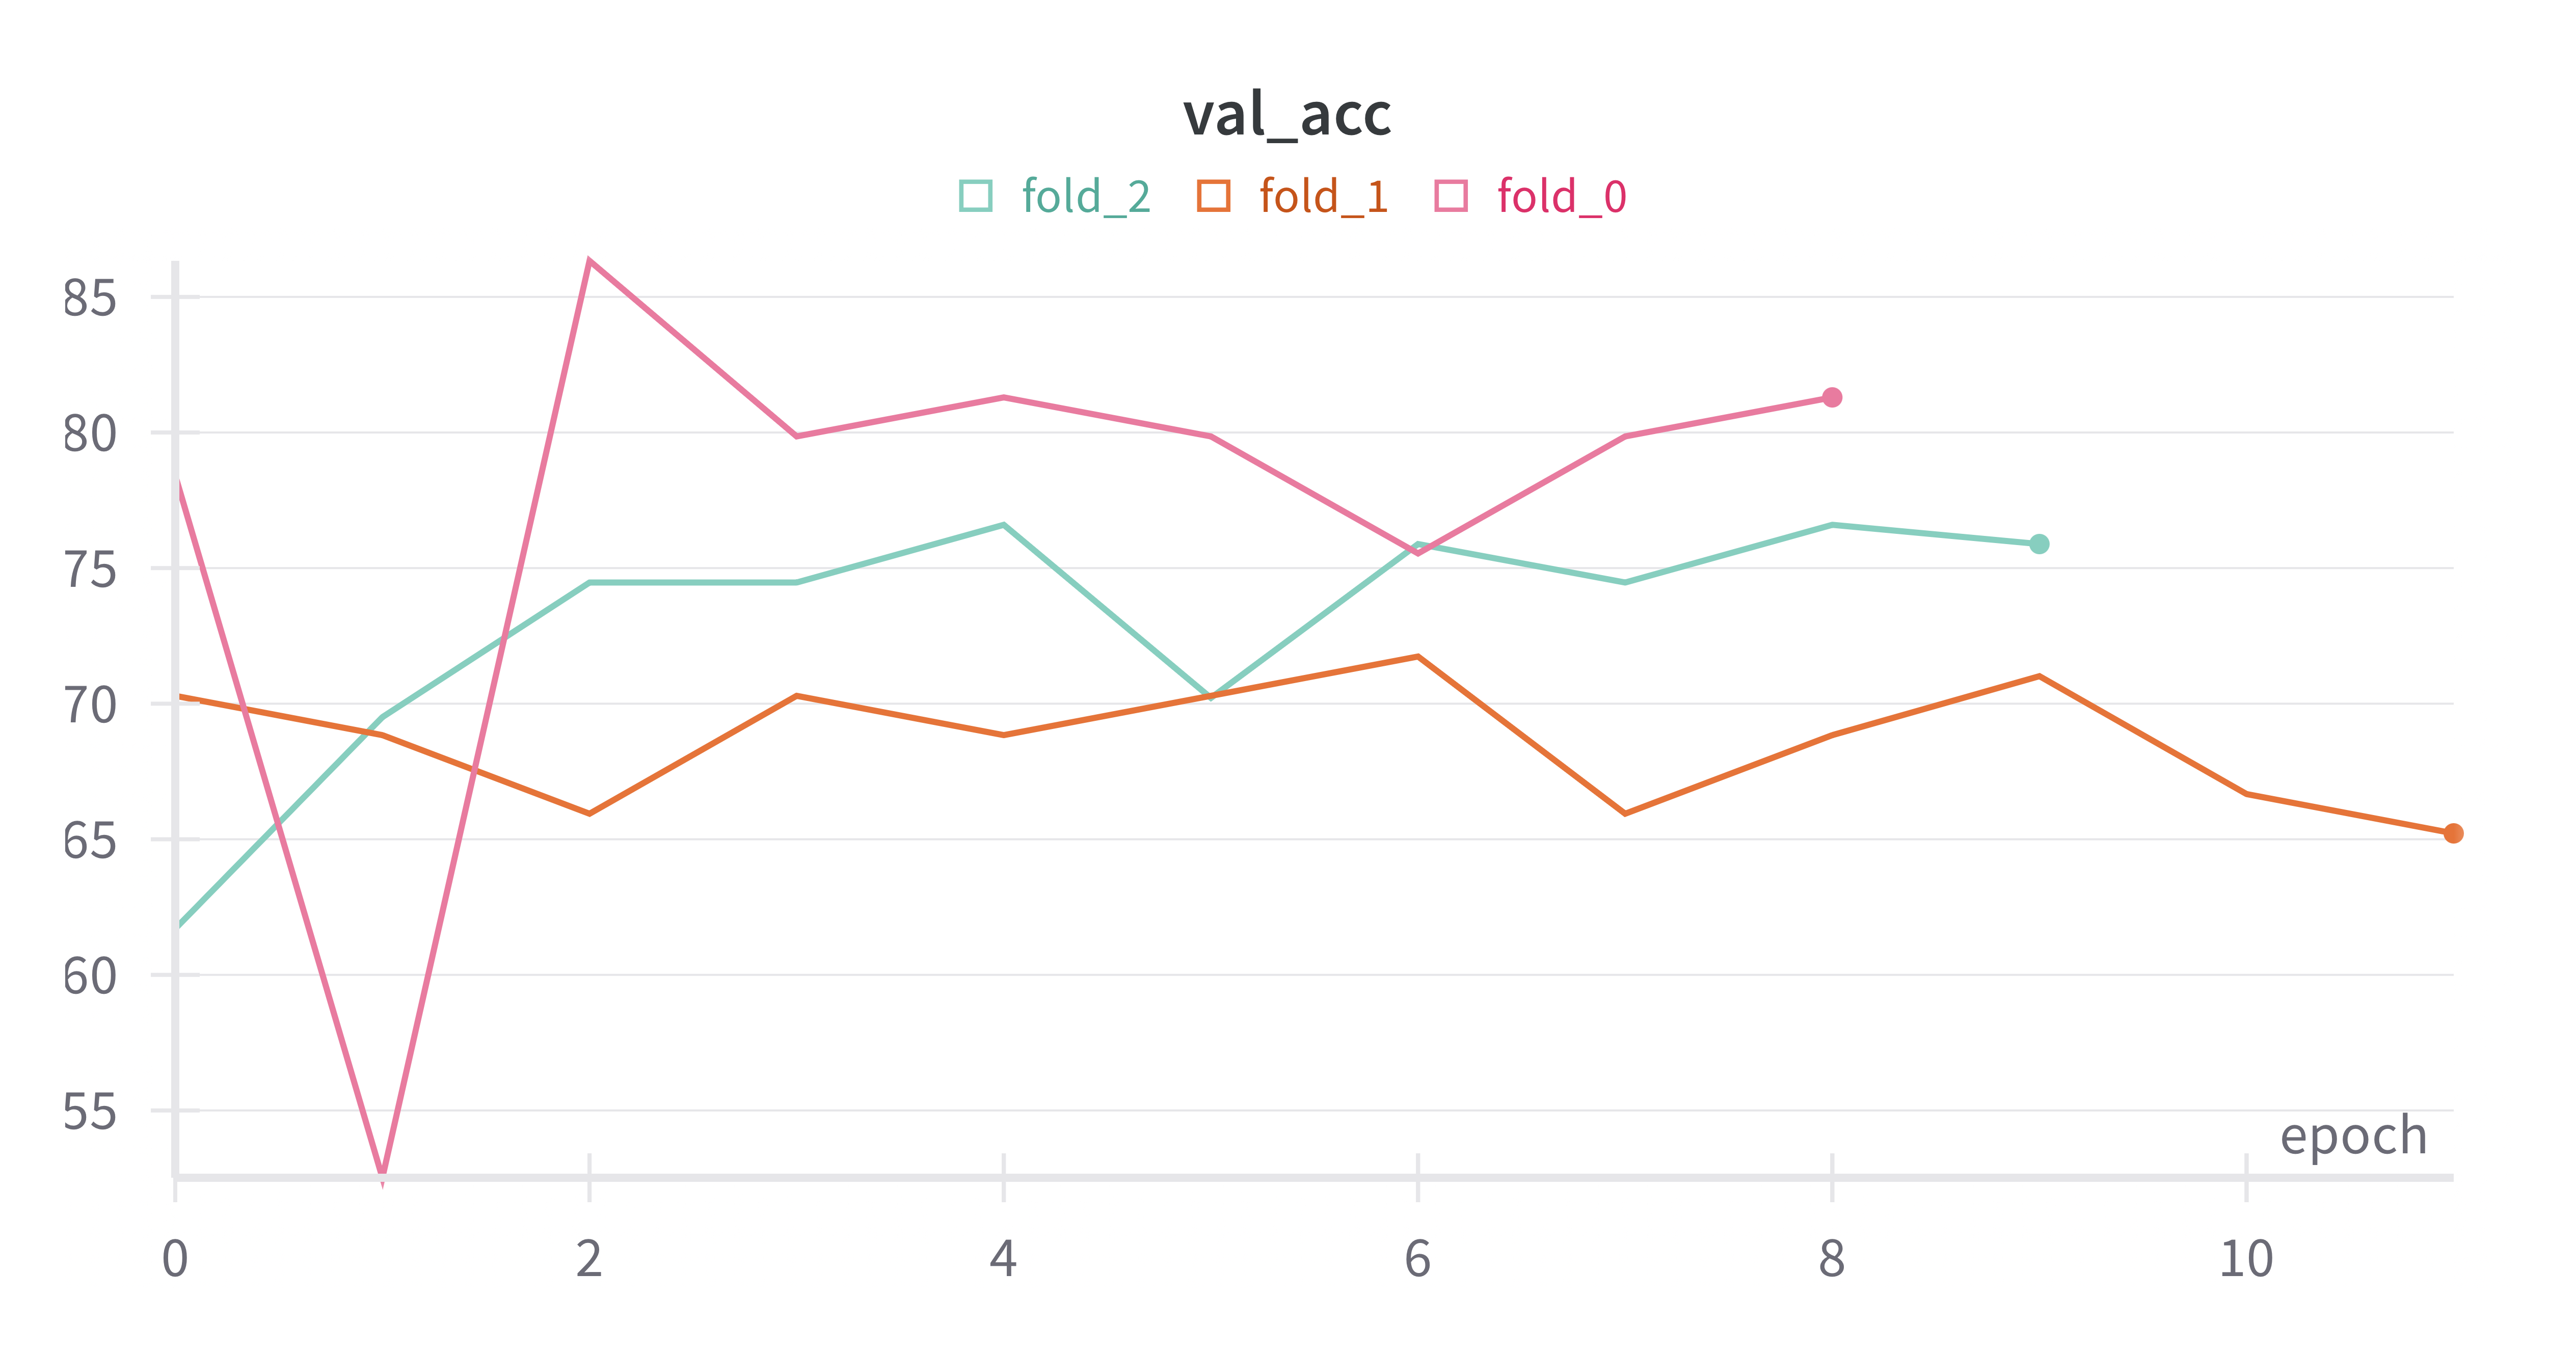
\includegraphics[width=0.6\textwidth]{figures/3f_val_acc.png}
  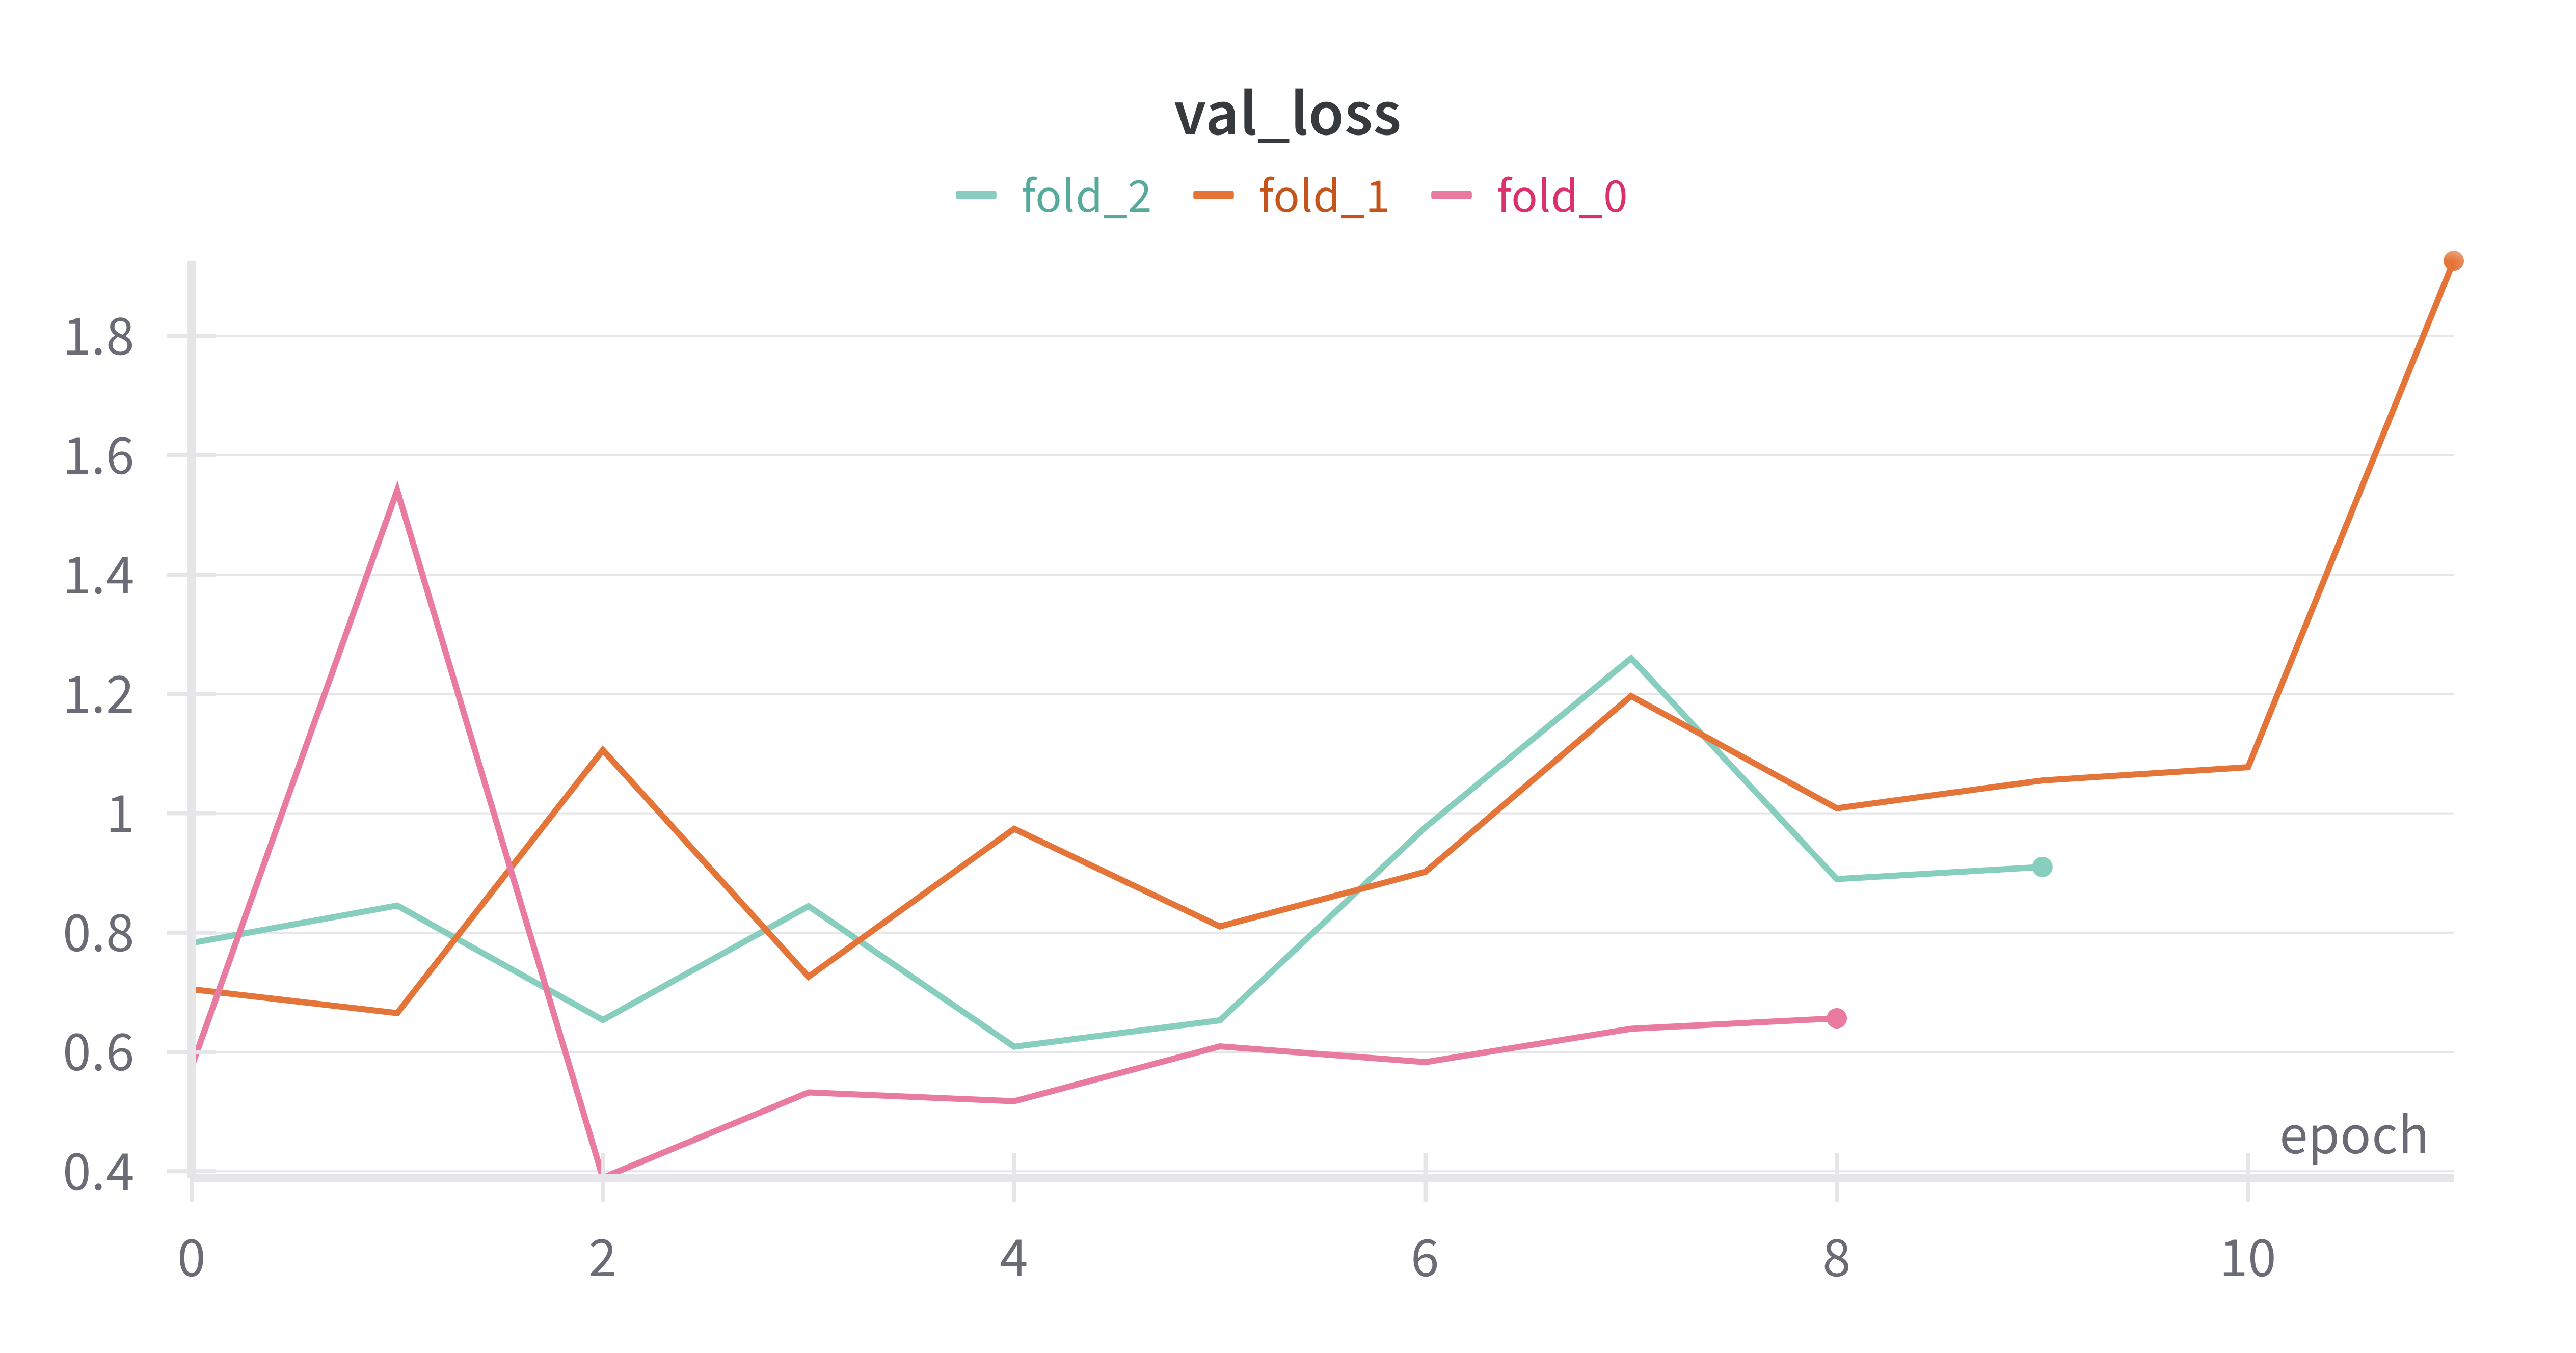
\includegraphics[width=0.6\textwidth]{figures/3f_val_loss.png}
  \caption{Learning curves showing training and validation loss/accuracy across epochs for the R3D-18 model.}
  \label{fig:learning_curves}
\end{figure}

The validation accuracy typically plateaued around epoch 5, after which the early stopping mechanism prevented overfitting by halting training when no further improvement was observed for 5 consecutive epochs.

\subsection{Architectural Comparisons}

\subsubsection{Dimensional Processing Impact}

A systematic comparison of different 3D architectural variants revealed a clear pattern: performance progressively declined as architectures incorporated more 2D elements. Figure \ref{fig:architecture_comparison_gl} and \ref{fig:architecture_comparison} illustrates this comparison across three main architectural approaches.
\begin{figure}[htbp]
  \centering
  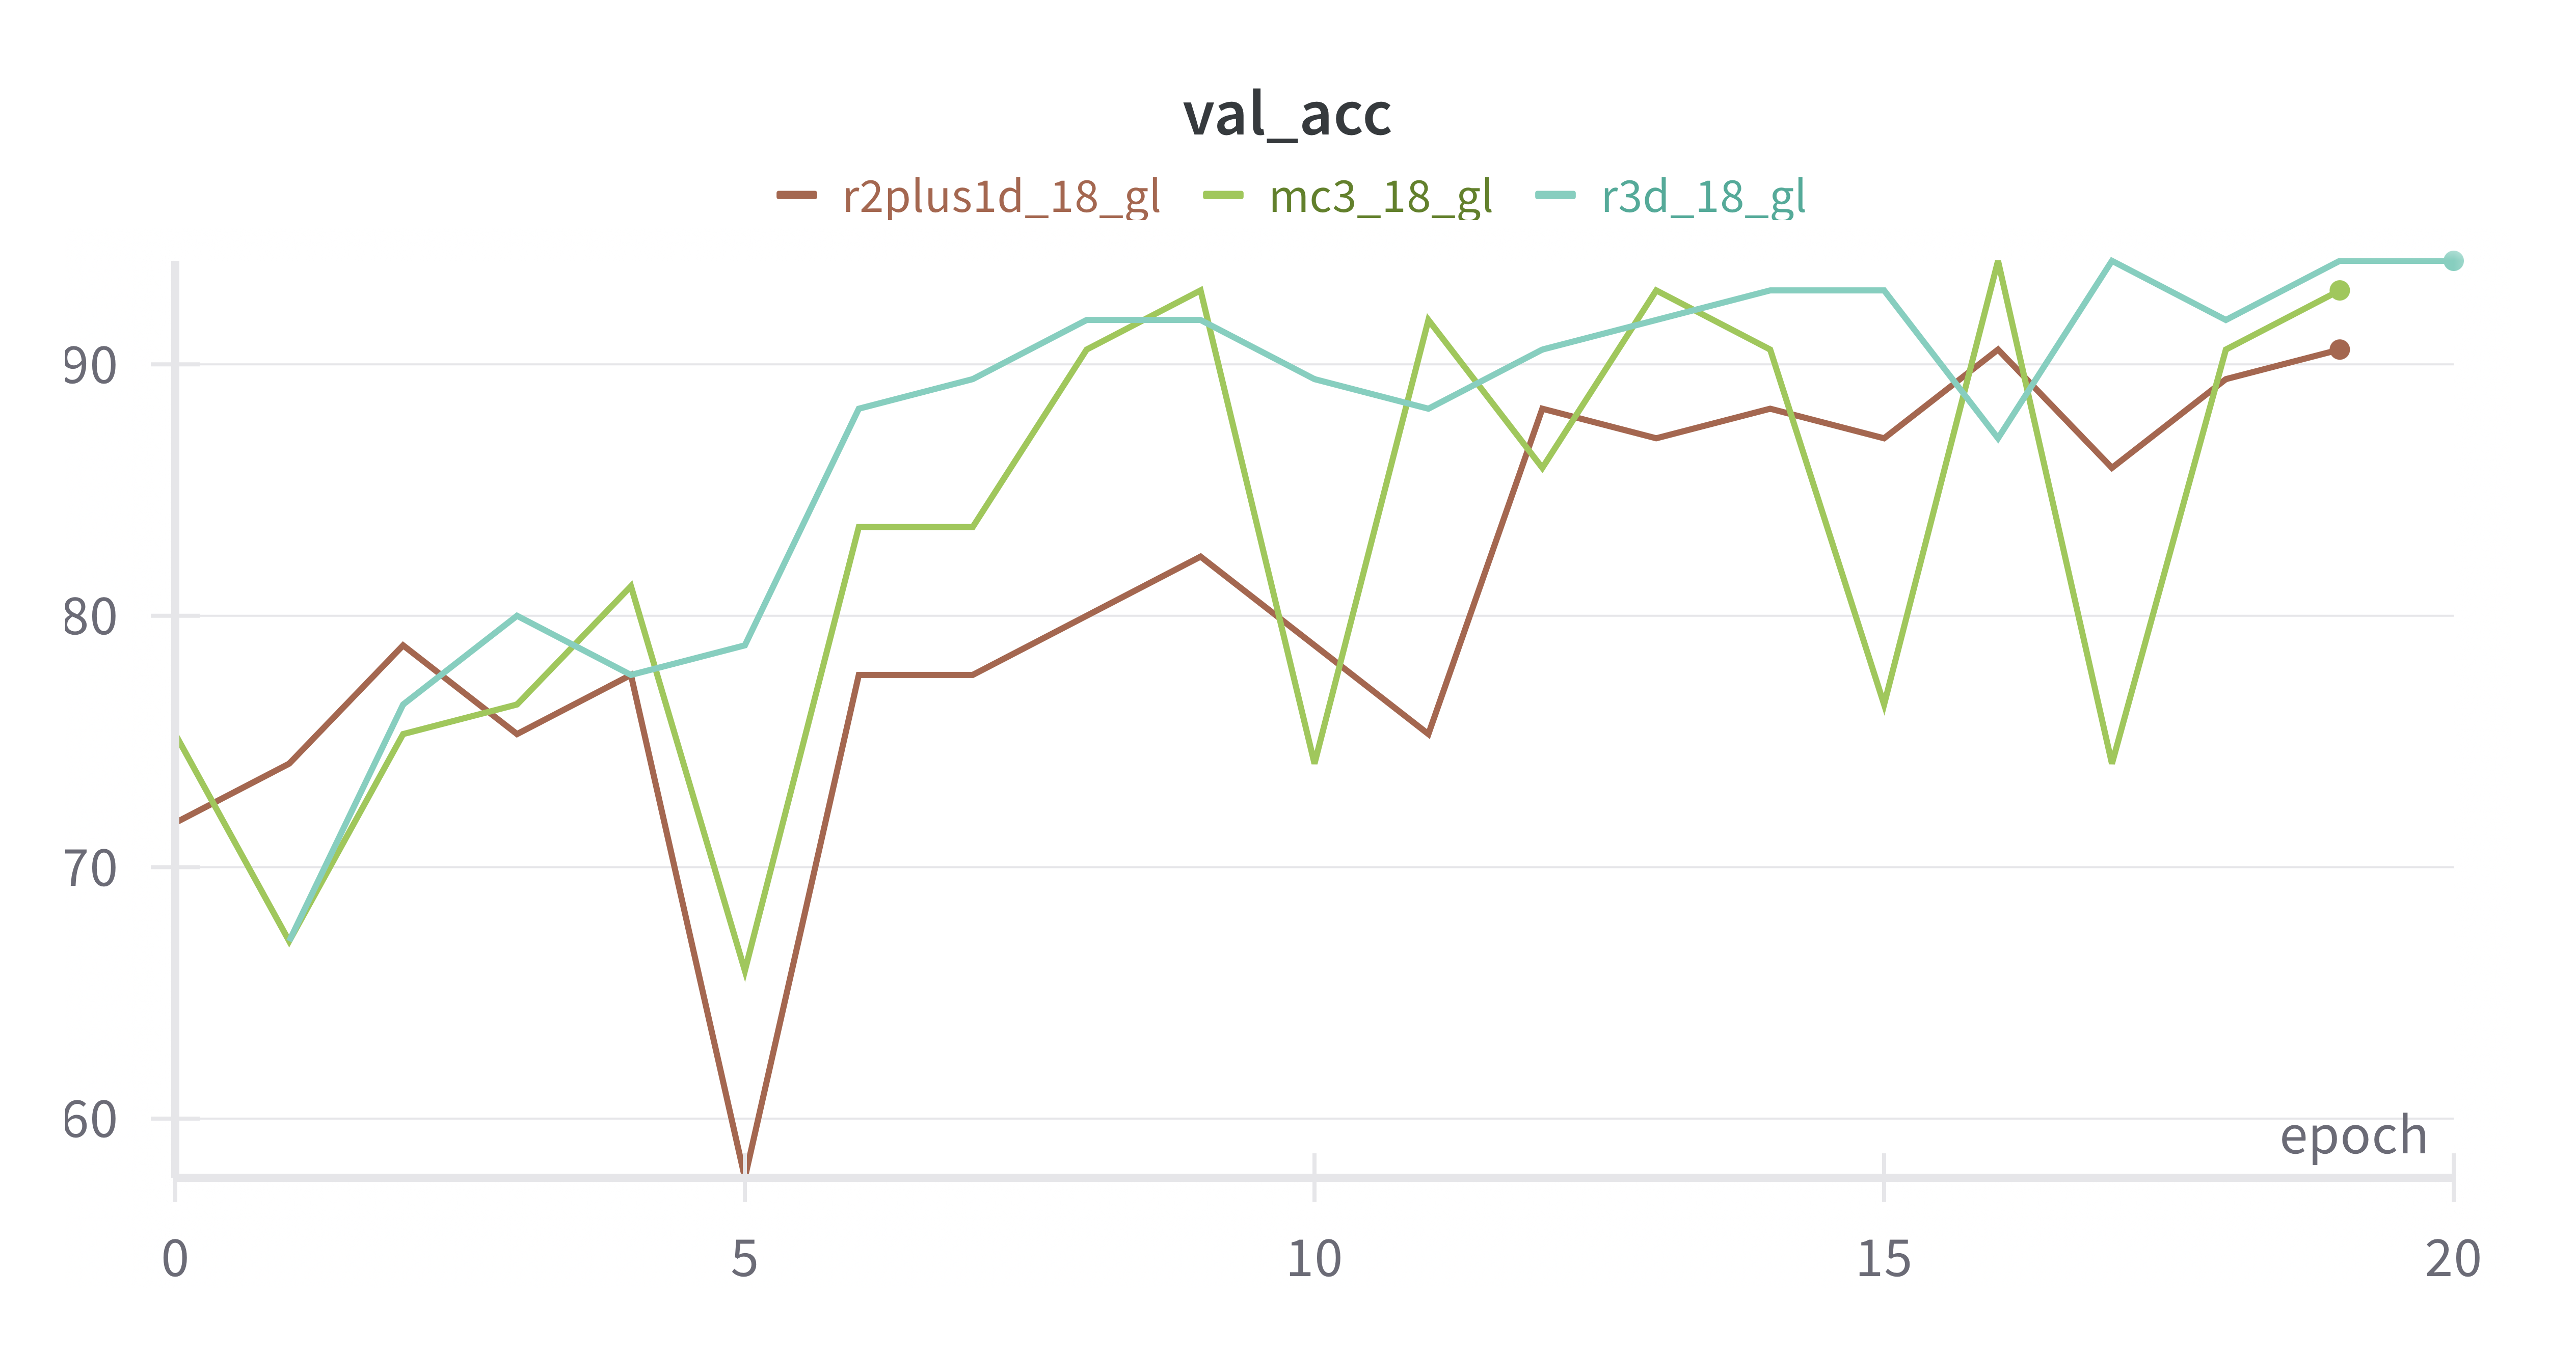
\includegraphics[width=\textwidth]{figures/archs_acc_gl.png}
  \caption{Performance comparison across architectural variants, demonstrating superior performance of fully 3D convolutional approaches (R3D-18) compared to hybrid architectures (MC3-18) and factorized convolutions (R(2+1)D-18). Note, group leakage was present in these runs, leading to inflated scores.}
  \label{fig:architecture_comparison_gl}
\end{figure}

\begin{figure}[htbp]
  \centering
  % TODO [INSERT ACTUAL ARCHITECTURE COMPARISON FIGURE]
  \caption{Performance comparison across architectural variants, demonstrating superior performance of fully 3D convolutional approaches (R3D-18) compared to hybrid architectures (MC3-18) and factorized convolutions (R(2+1)D-18). Note, no group leakage was present in these runs.}
  \label{fig:architecture_comparison}
\end{figure}

The fully 3D convolutional approach (R3D-18) consistently outperformed both the mixed convolution network (MC3-18) and the factorized convolutional approach (R(2+1)D-18), with test accuracies of 97.67\%, 93.02\%, and 94.18\% respectively, these figures are inflated due to group leakage, after correcting for group leakage we saw test accuracies of 79.14\%, 67.63\%, and xxx\% respectively. This progression strongly suggests that preserving complete 3D spatial context is critical for effective AD classification from volumetric MRI data.

% TODO add actual r2plus1d values and figure

\subsubsection{Layer Freezing Strategy Analysis}

Experiments with different layer freezing strategies revealed significant impact on model stability and performance. Table \ref{tab:freezing_strategies} summarizes these findings.

\begin{table}[htbp]
\centering
\begin{tabular}{|l|c|c|p{4cm}|}
\hline
\textbf{Strategy} & \textbf{Trainable Parameters} & \textbf{Result} & \textbf{Observation} \\
\hline
FC layer only & 0.003\% (1,026) & Failed training & Numerical instability (NaN losses) \\
\hline
FC + Layer 4 & 75.15\% (24.9M) & Successful & Best balance of stability and performance \\
\hline
Full fine-tuning & 100\% (33.1M) & Successful & Increased overfitting risk, slower convergence \\
\hline
\end{tabular}
\caption{Comparison of different layer freezing strategies and their impact on training stability and performance.}
\label{tab:freezing_strategies}
\end{table}

Notably, attempting to train only the final fully connected layer (preserving 99.997\% of pre-trained weights) resulted in numerical instability, suggesting that significant domain adaptation is necessary for the substantial shift from video action recognition to MRI classification. The optimal approach (FC + Layer 4) balanced stable training with effective knowledge transfer.

\subsection{Preprocessing Impact Analysis}

\subsubsection{Impact of Crop-and-Reshape Strategy}

The adaptive cropping strategy yielded substantial performance improvements compared to naive interpolation. As shown in Figure \ref{fig:cropping_impact}, the accuracy differential between models trained on 96³ naively interpolated volumes versus 128³ adaptively cropped volumes was significant.

\begin{figure}[htbp]
  \centering
  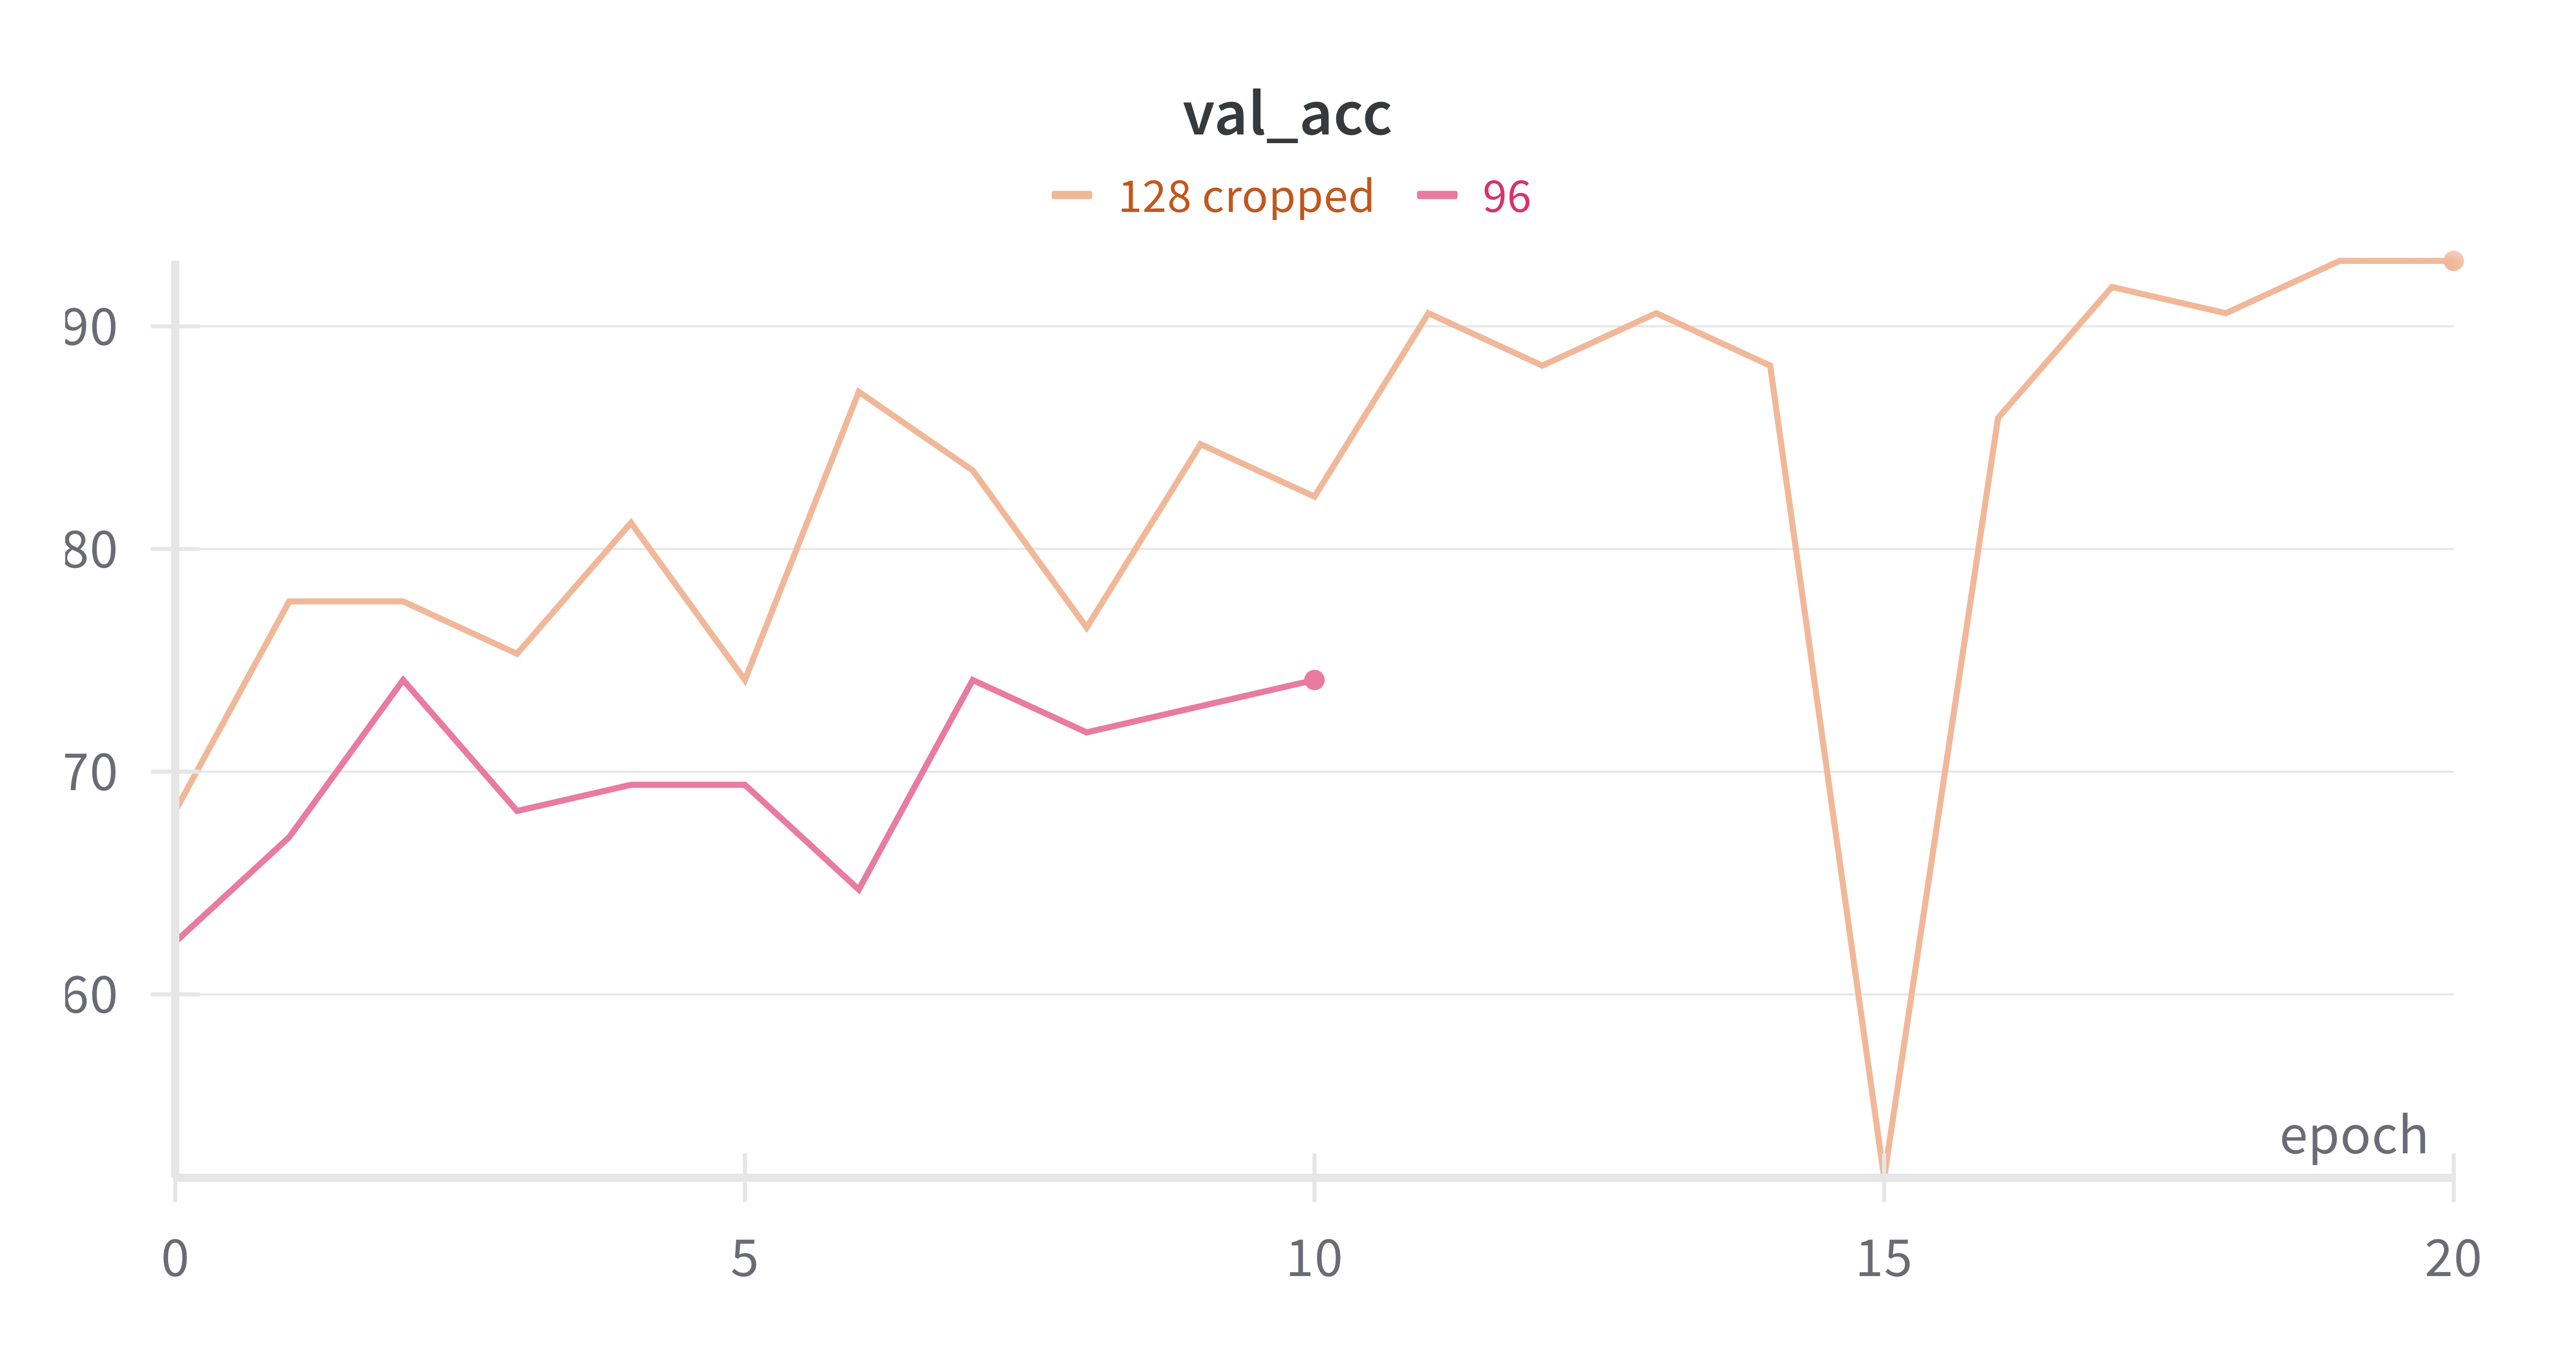
\includegraphics[width=0.8\textwidth]{figures/crop_val_acc.png}
  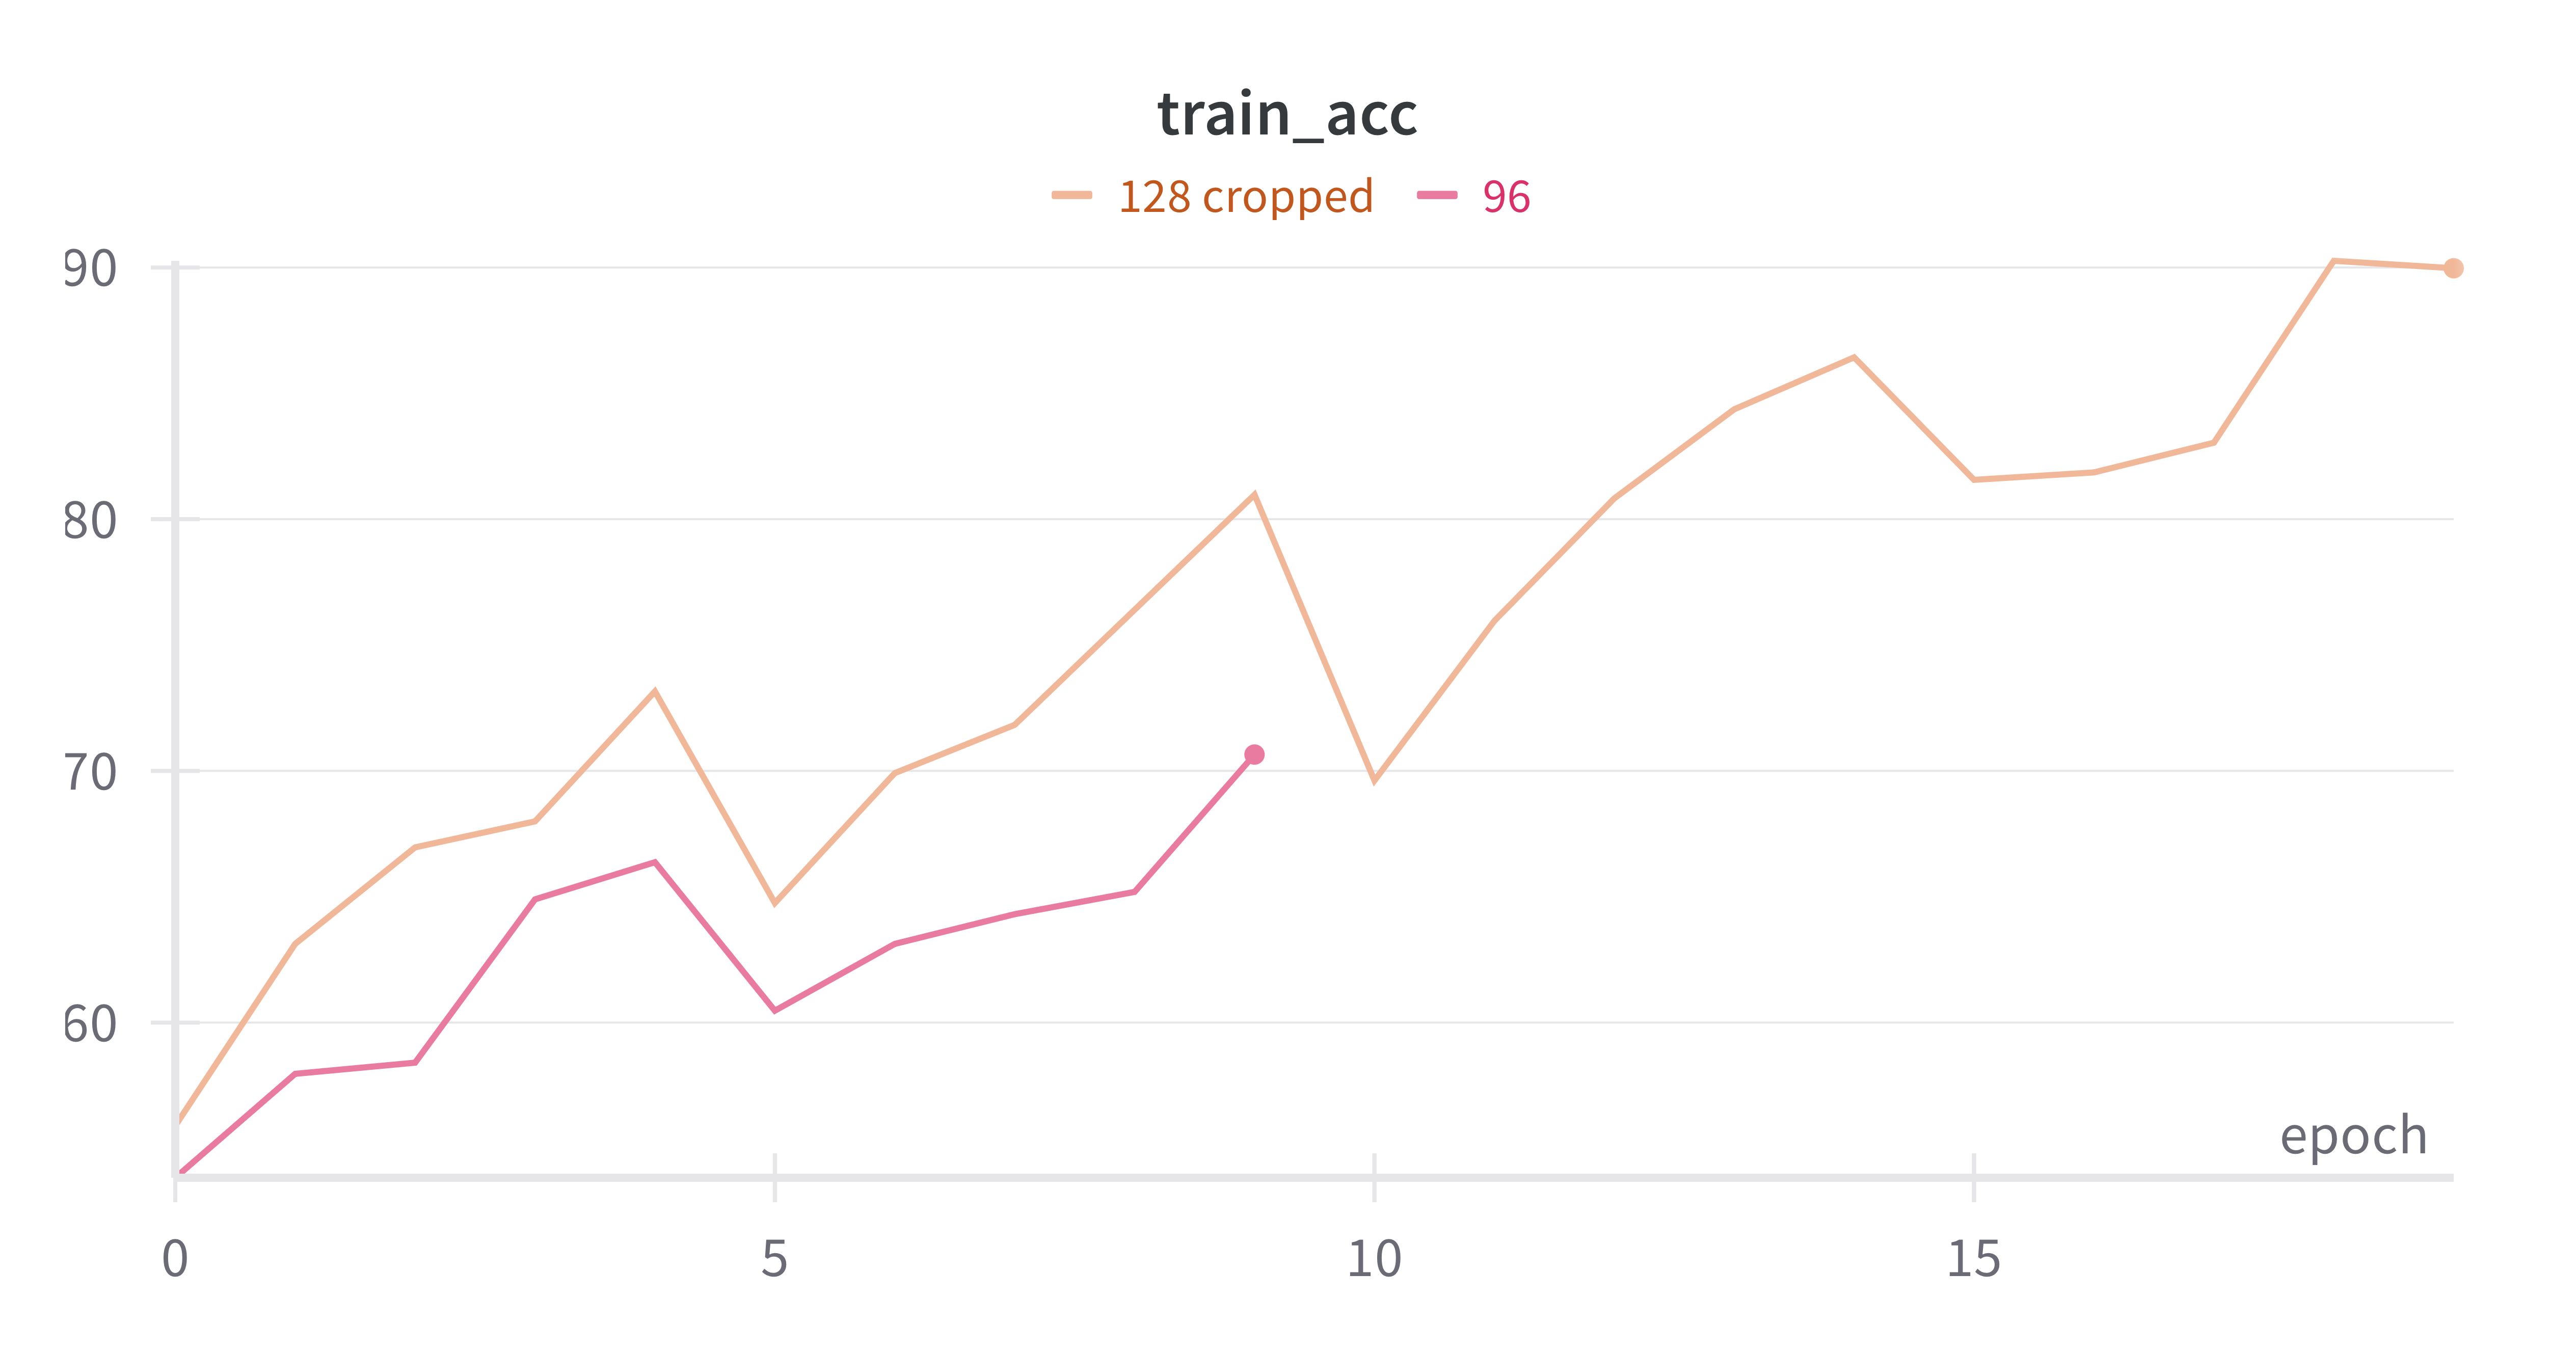
\includegraphics[width=0.8\textwidth]{figures/crop_train_acc.png}
  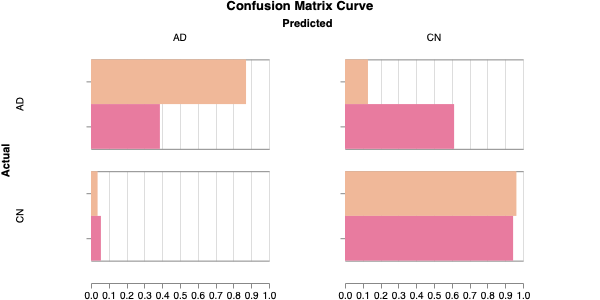
\includegraphics[width=0.8\textwidth]{figures/crop_CM.png}
  \caption{Performance comparison between naive downsampling (96³) and adaptive cropping with higher resolution (128³), demonstrating the importance of preserving anatomical detail. Note: This inflated accuracy is due to group leakage having not yet been implemented, but all else is equal despite the 96³ vs 128³ difference.}
  \label{fig:cropping_impact}
\end{figure}

This improvement can be attributed to the preservation of approximately 35\% more effective resolution for critical structures like the hippocampu as well as a 2.37x increase in resolution, allowing the model to better detect subtle atrophy patterns characteristic of AD.

\subsubsection{Skull Stripping Quality}

SynthStrip was selected as the skull stripping method for all preprocessing due to its known advantages in handling atrophied brains. While a direct comparison between skull stripping methods was not performed, qualitative assessment of the SynthStrip results showed excellent preservation of cortical boundaries and consistent handling of atrophied brain regions characteristic of Alzheimer's disease. Figure \ref{fig:skull_stripping_comparison} shows example outputs from SynthStrip, demonstrating its effectiveness across different subjects in our dataset.

The literature suggests that high-quality skull stripping is important for AD classification tasks, with previous studies reporting performance differences of 2-4\% between optimal and suboptimal brain extraction methods \cite{hoopes2022synthstrip}. By employing SynthStrip consistently across all scans, non-brain tissue did not introduce confounding signals that might otherwise impact the model's ability to identify disease-specific patterns.

\begin{figure}[htbp]
  \centering
  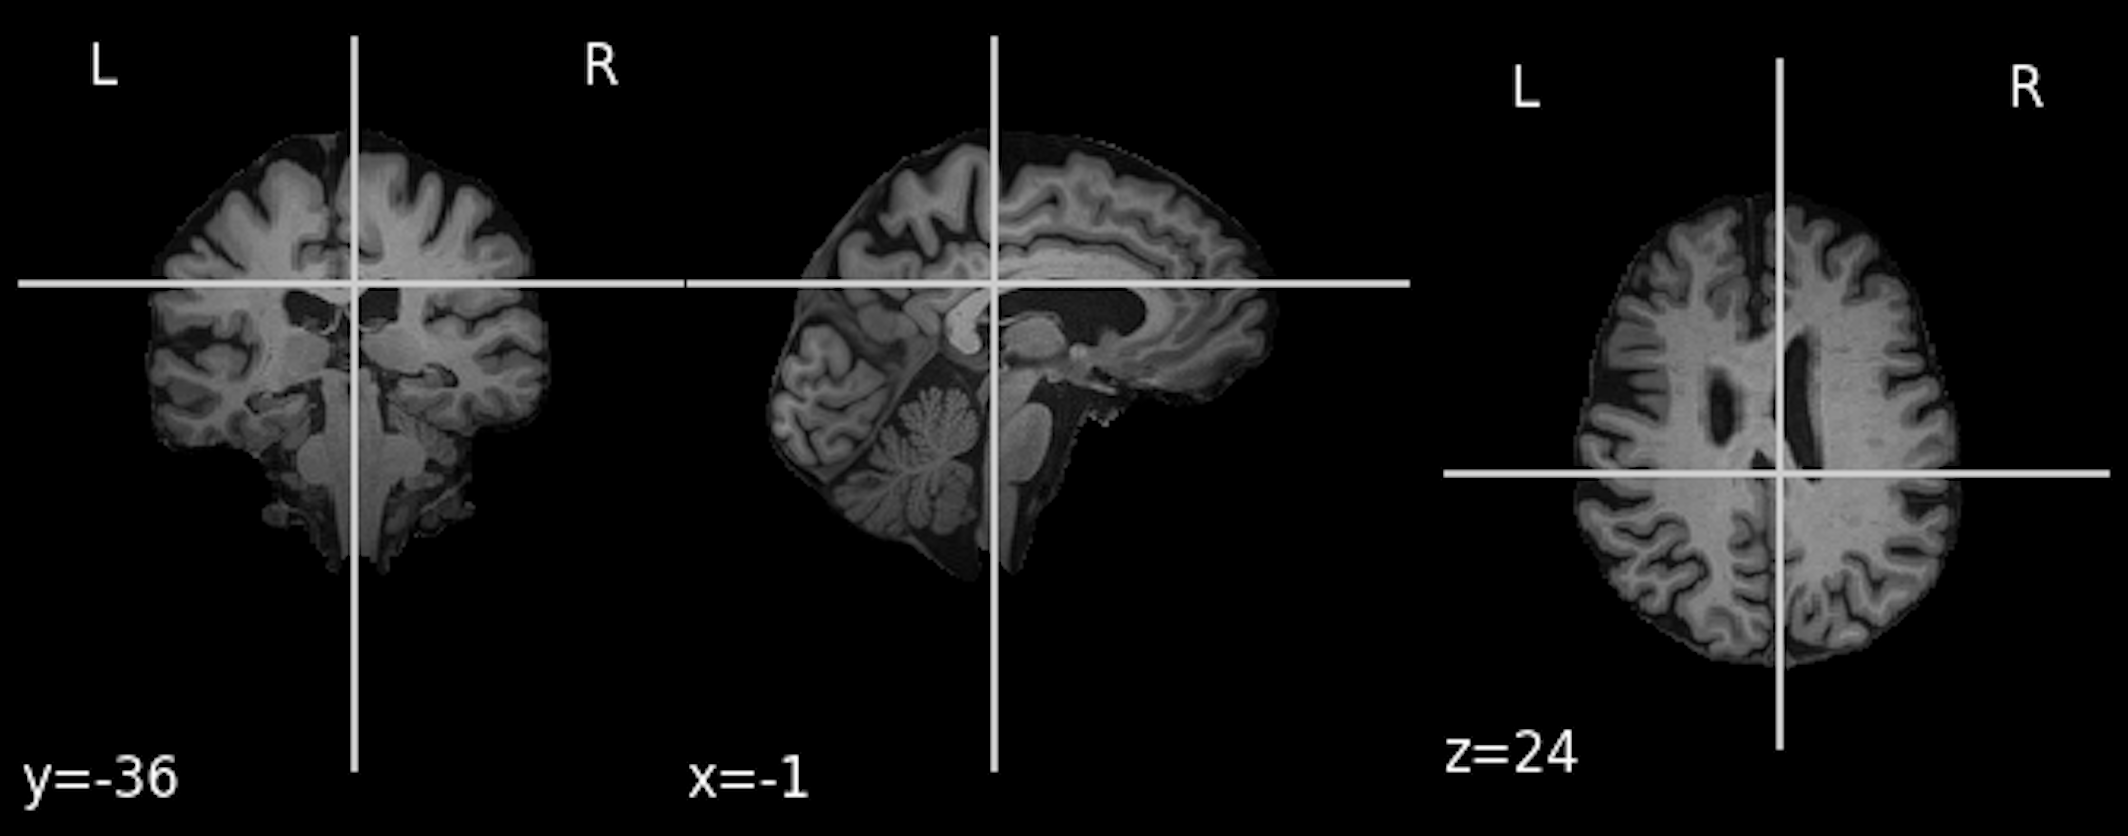
\includegraphics[width=\textwidth]{figures/ss.png}
  \caption{Example SynthStrip output.}
  \label{fig:skull_stripping_comparison}
\end{figure}

\subsection{Augmentation Effectiveness}

\subsubsection{Comparative Analysis of Augmentation Strategies}

Through systematic experimentation, it was identified that minimal, targeted augmentation outperformed more extensive transformation sets. Figure \ref{fig:augmentation_comparison} illustrates the performance impact of different augmentation strategies. $tio_s$ and $tio_l$ being torchio augmentations with smaller and larger values, the augmentations include rotations, translations, random noise, gamma adjustment, and z-normalization, showing the effectiveness of minimalist approach focusing on noise, gamma adjustment, and normalization versus more extensive transformations. $tio_flip$ was $tio_s$ plus flips, and $monai$ was using similar augmentations to $tio_flip$ but using the monai library.

\begin{figure}[htbp]
  \centering
  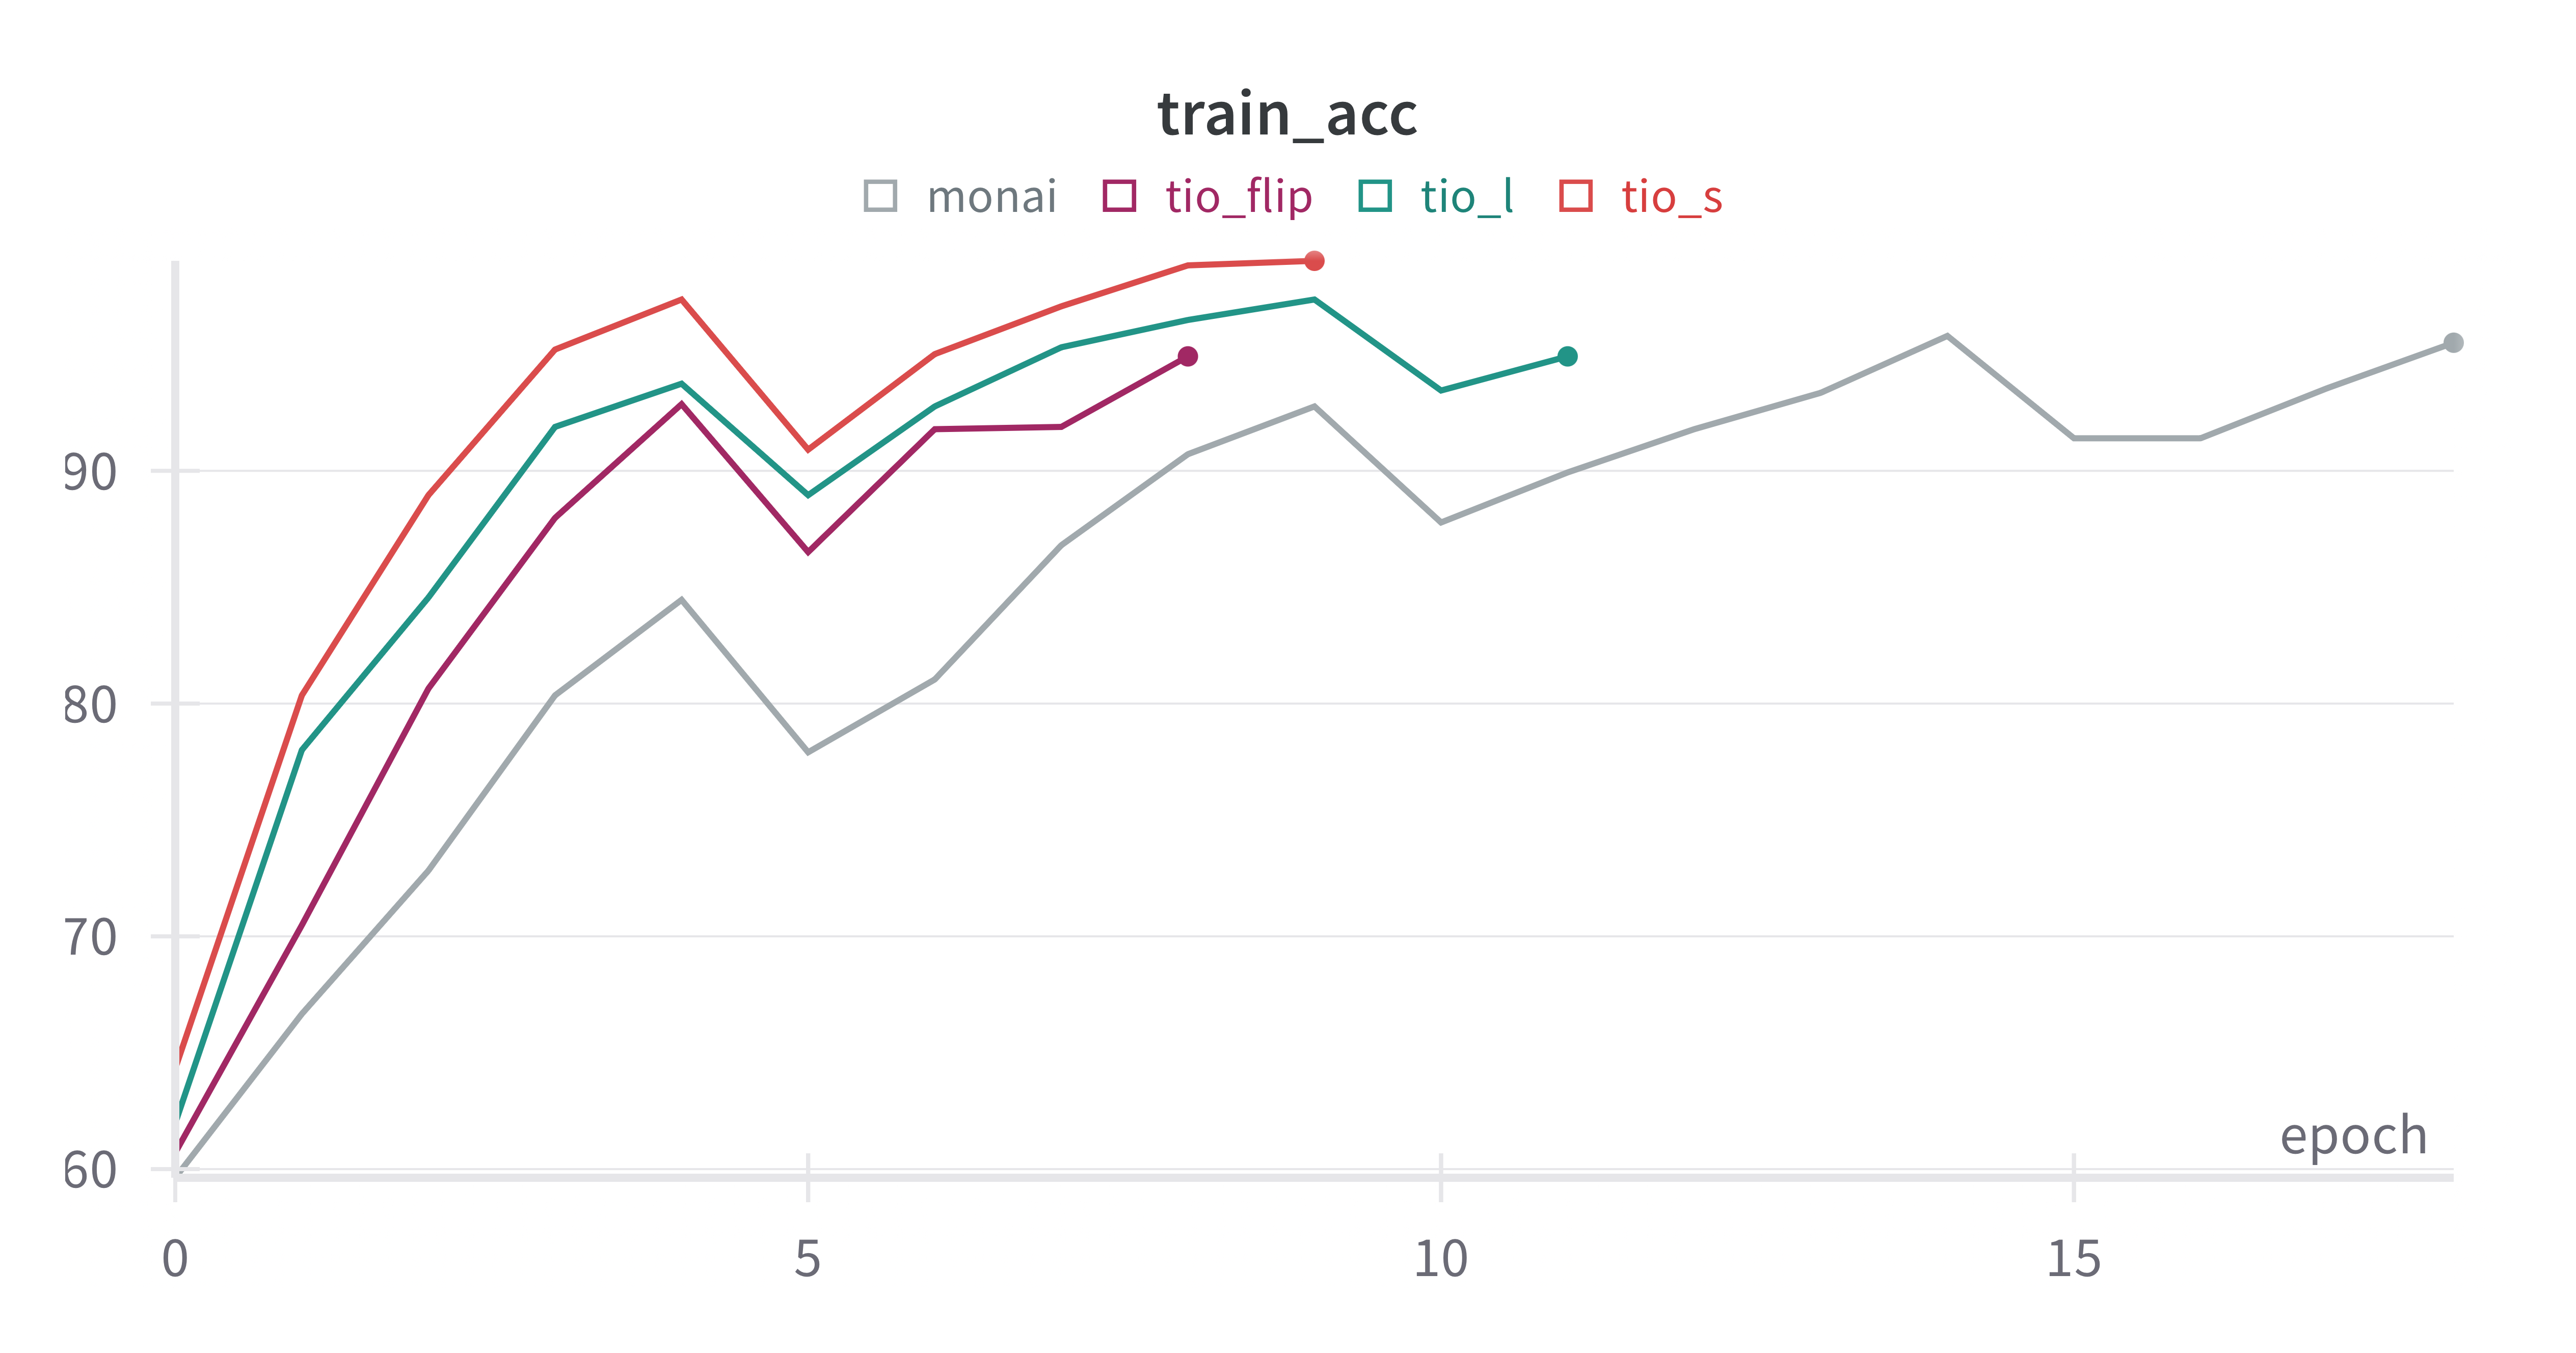
\includegraphics[width=\textwidth]{figures/augs_train_acc.png}
  \caption{Training accuracy performance comparison across different augmentation strategies.}
  \label{fig:augmentation_comparison}
\end{figure}

The optimal strategy (random noise + gamma adjustment + Z-normalization) improved validation accuracy by approximately 5\% compared to using no augmentation, while the addition of geometric transformations (rotations, flips) not only failed to improve performance, as they all remaied within ±2\% but significantly increased training time from approximately 5 to 20 epochs for comparable convergence.

\subsubsection{Normalization Impact}

Z-normalization proved particularly effective, as demonstrated in Figure \ref{fig:normalisation_accuracy} which shows the consistent improvement in validation accuracy as well as a more stable convergence when normalization was included in the augmentation pipeline.

\begin{figure}[htbp]
  \centering
  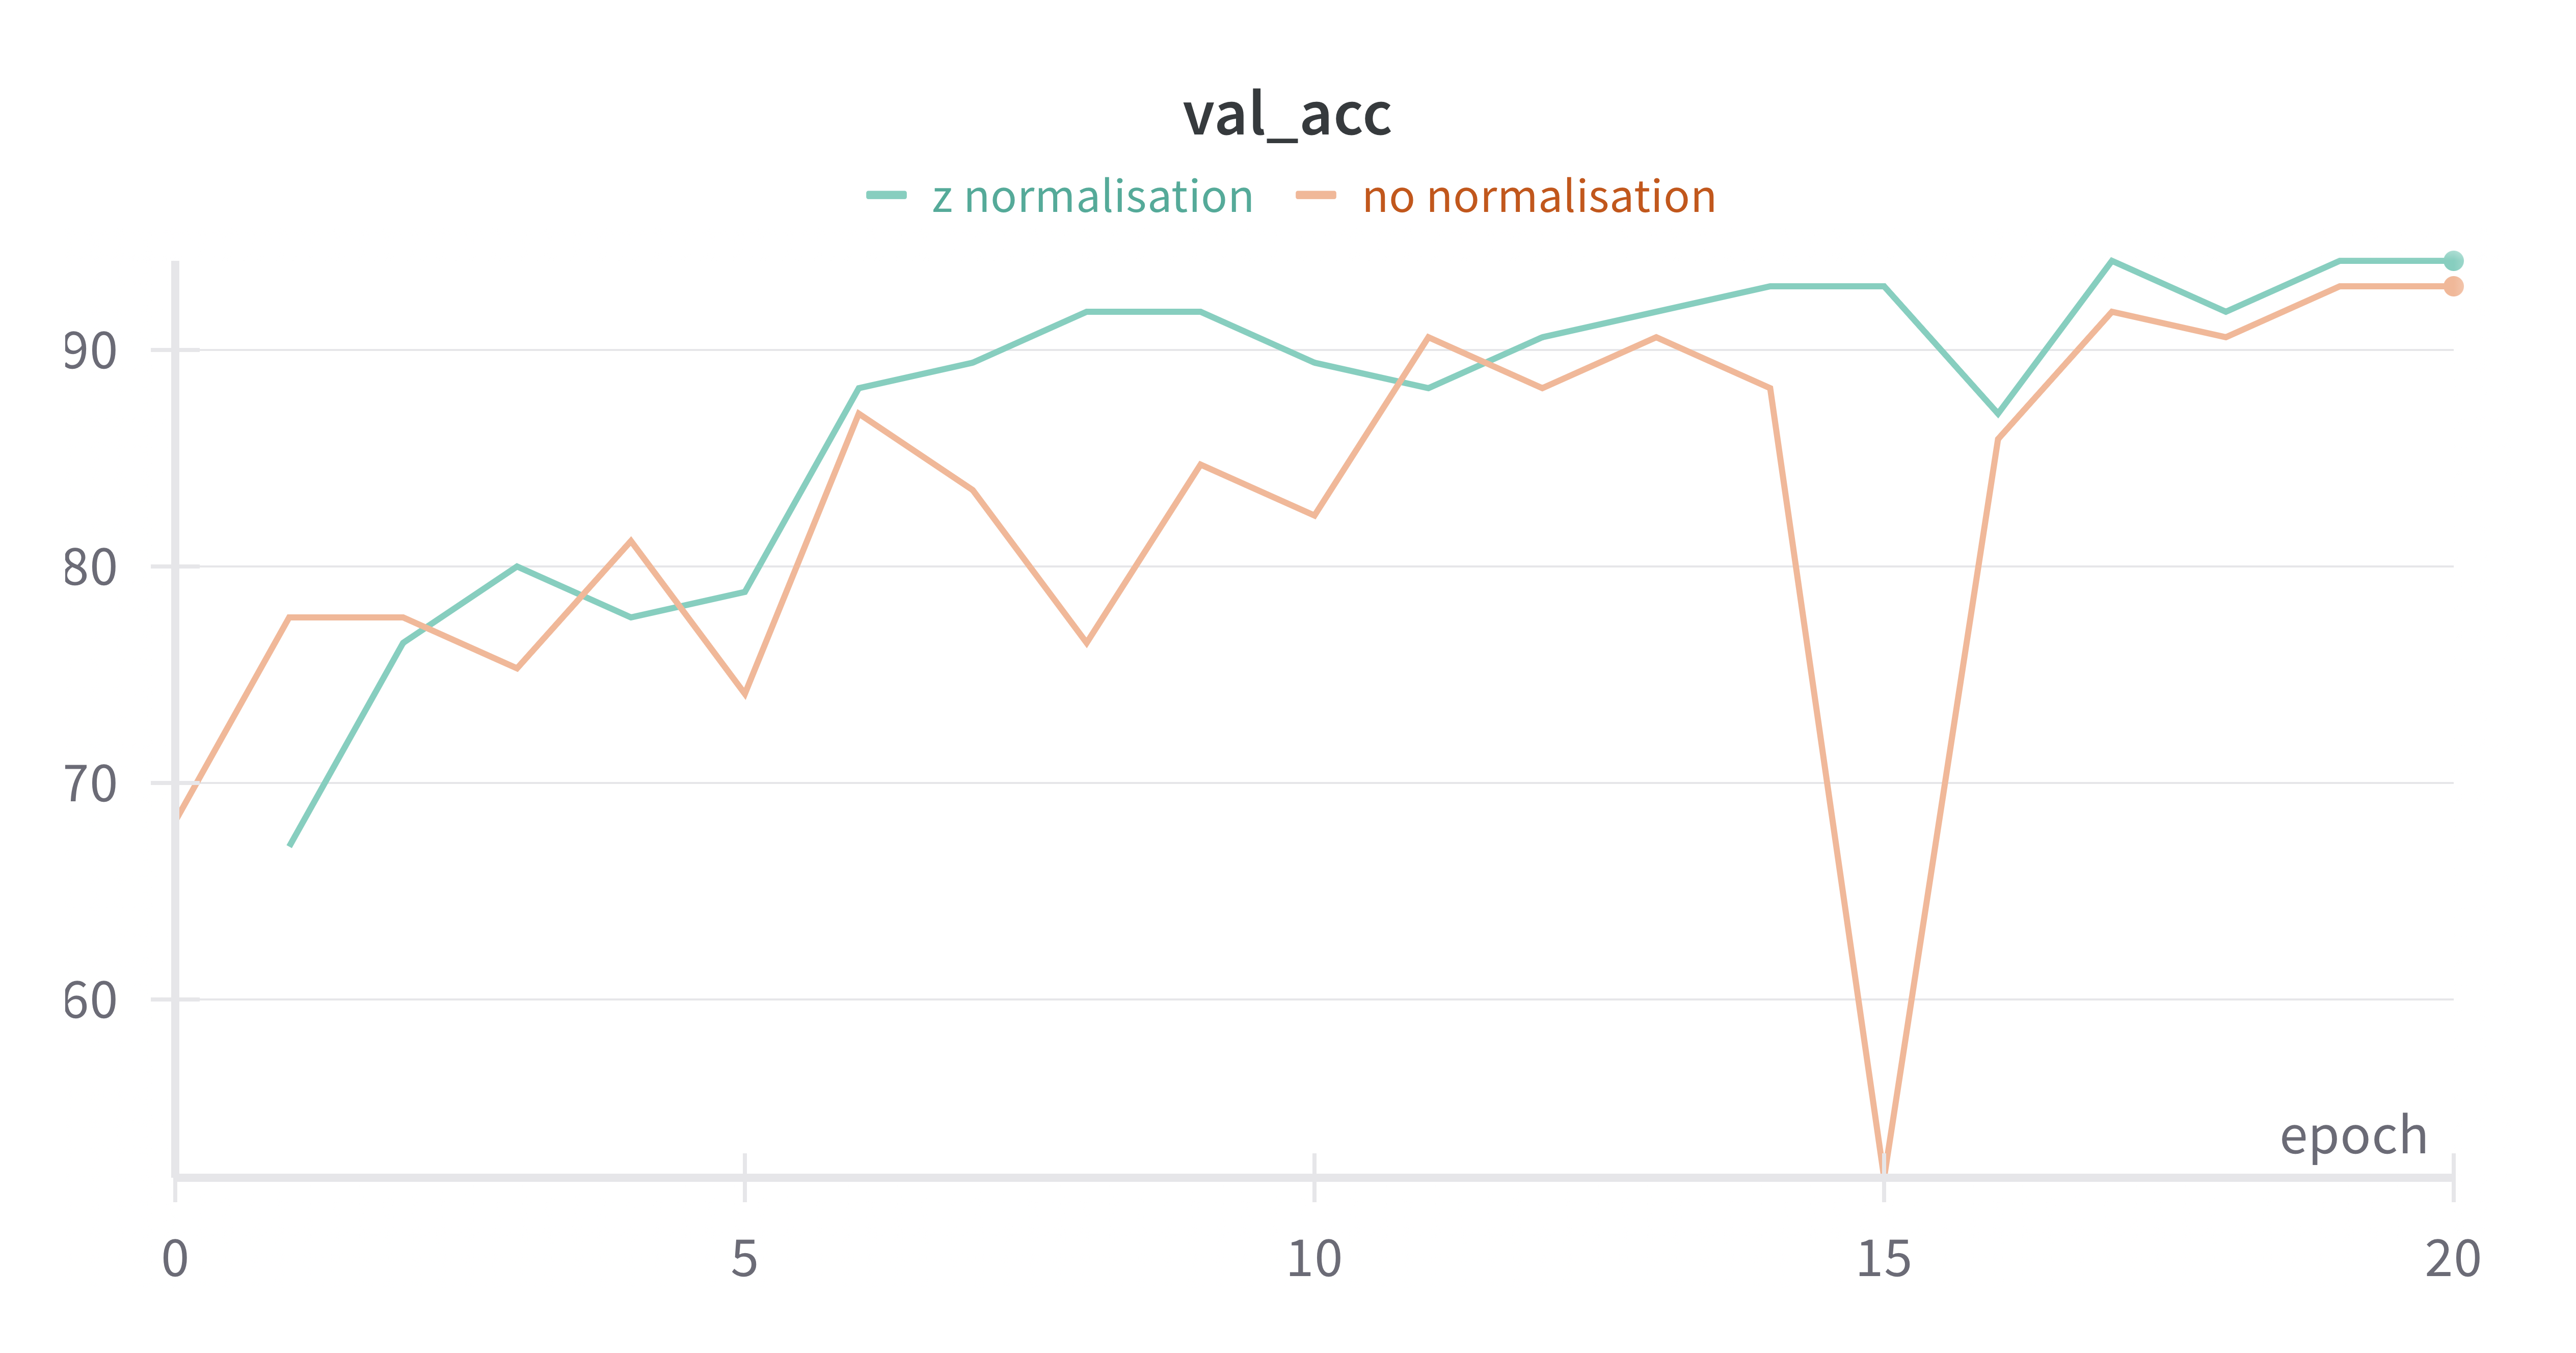
\includegraphics[width=\textwidth]{figures/znorm_val_acc.png}
  \caption{Validation accuracy over epochs with and without normalisation in the augmentation, demonstrating normalisations effectiveness in enhancing model generalization.}
  \label{fig:normalisation_accuracy}
\end{figure}

\section{Discussion}
% 2,000 words

% - **Interpretation of Results**

%   - Critical analysis of performance metrics
%   - Analysis of 77% accuracy in clinical context
%   - Comparison with human radiologist performance
%   - Significance relative to existing literature
%   - Analysis of false positives and false negatives

% - **Technical Insights**

%   - Effectiveness of transfer learning from video domain
%   - Value of 3D vs. 2D/3D hybrid approaches
%   - Computational efficiency considerations
%   - Memory constraints and their implications

% - **Model Interpretability** (if implemented)

%   - Insights from XAI analysis
%   - Visualization techniques for model attention/activation
%   - Correlation with known AD-affected regions
%   - Clinical relevance of identified features

% - **Clinical Implications**

%   - Potential utility as a diagnostic aid
%   - Integration into existing clinical workflows
%   - Complementary role to other diagnostic measures

% - **Technical Challenges and Solutions**

%   - Memory optimization strategies
%   - Training time challenges on consumer hardware
%   - Data preprocessing optimization
%   - Hardware limitations and workarounds
%   - Data leakage prevention and subject isolation

% - **Limitations**
%   - Dataset representativeness and potential biases
%   - Focus on binary classification (AD vs. CN)
%   - Technical constraints (resolution, model capacity)
%   - Hardware constraints impact on model selection
%   - Need for prospective validation
%   - Generalizability concerns

\section{Conclusions}
% 1,000 words

% - **Summary of Contributions**

%   - Key findings on transfer learning effectiveness
%   - Revisiting research objectives
%   - Technical innovations in preprocessing pipeline
%   - Methodological contributions (subject-level validation)

% - **Future Directions**

%   - Architectural improvements
%   - Multi-class classification (including MCI)
%   - Multimodal approaches
%   - Longitudinal analysis potential
%   - Clinical validation pathway
%   - Integration of additional MRI sequences
%   - Consideration of larger/deeper architectures with more compute

% - **Broader Impact**
%   - Implications for AI in neuroimaging
%   - Potential for improving AD diagnosis workflow
%   - Ethical considerations and responsible deployment

\bibliographystyle{IEEEtran}
\bibliography{references} 

\appendix

% - **Detailed Implementation Specifics**

%   - Code snippets for key components
%   - Hyperparameter configurations
%   - Detailed architectures

% - **Additional Visualizations**

%   - Extended results tables
%   - Additional performance metrics
%   - Sample preprocessing visualizations
%   - Extended XAI visualizations

% - **Computational Resources Analysis**
%   - Detailed training times
%   - Memory usage patterns
%   - Optimization attempts


\end{document}



